% Ensamblado del artículo VII, revisión de integración 07.
% Título y tres movimientos conservados en PROPUESTA_EDITORIAL.md.
% Núcleo común conservado literalmente y antecedentes copiados de V REV02.
% El cierre textual de inputs no sustituye la validación de todas sus pruebas.
% La amplitud material y su dominio se demuestran en el fragmento 33.
% La entrega exige además preflight, compilación y comprobación visual.
% Artículo VII — primera redacción editorial, 10 de septiembre de 2026.
% Apertura integrada con las demostraciones de la revisión 06.
% Procedencia y condiciones: PLAN_RESIDENCIAS_DEMOSTRATIVAS.md.
% Las referencias internas remiten a demostraciones incluidas en el cuerpo.

\begin{center}\bfseries Resumen\end{center}
\begingroup
\fontsize{10}{12}\selectfont
\setlength{\parskip}{2pt plus 1pt minus .5pt}
\noindent
Se determina la amplitud torsional como funcional explícito del estado
material mediante la acción espinorial, la eliminación de la contorsión
y la variación métrica. Se construye un sector material en el que esa
amplitud es positiva y se conserva. Su contribución energética produce
una dilución \(a^{-6}\) y, en la realización homogénea plana con
\(\Lambda_{\mathrm{eff}}=0\), densidades positivas y \(w<1\), un umbral
de rebote único y transversal. Para polvo se obtiene una solución exacta
para todo tiempo, con curvatura finita y geodésicas causales de
Levi--Civita completas en ambas direcciones.

La construcción parte de un núcleo formal denominado Holografía Modular
Triádica, en adelante HMT. \emph{All Possible Paths}, en adelante APP,
reúne caminos aritméticos sobre \((\mathbb Z/9\mathbb Z)^2\), con
adyacencia dada por el grafo de Cayley aditivo de generadores cardinales
y realización celular toroidal, distinguiendo las operaciones y las
evaluaciones de suma y producto;
TRIT es la unidad de firma orientada \(\{-1,0,+1\}\) que determina los
regímenes locales; el \emph{Topological Phase Kernel}, en adelante TPK,
compone la dinámica de transporte y memoria. El estado enriquecido
conserva hojas, orientación, residuo, acarreo e historia durante el
retorno de fase. La Mecánica Dimensional expresa sus resultados
internos mediante magnitudes y observables físicos, preservando la
procedencia estructural de los acoplamientos.

La normalización gravitatoria se desarrolla previamente mediante la
composición longitudinal \(L=(5759/23040)\alpha^{16}L_*\) y su
métrica radial positiva. En la realización definida por esas operaciones
y por la identificación del radio gravitatorio reducido, la reciprocidad
con la sección de acción fija \(G=c^3L^2/\hbar_{\rm ret}\) en todos
los modos admisibles. La demostración conserva el archivo completo y
establece las condiciones de reducción estática y dinámica de la memoria.
La elección dimensional \(L_*=1\,\mathrm m\), las reglas longitudinal
y métrica y la identificación radial se declaran en el propio enunciado.

El transporte de rutas admite una realización de Cartan compatible con
composición, inversión y refinamiento. Sobre ella se distinguen dos
acciones materiales: la extensión minimizante de la pantalla de memoria
y la realización espinorial. Cada una conserva su propia variación
respecto de la conexión. En el sector espinorial, afín en la contorsión,
la inversión de los operadores de Holst y torsión determina la corrección
efectiva; para la extensión mínima se conserva la dependencia no lineal
de la corriente y se demuestra un criterio local mediante el Hessiano.
La corriente, el observable cuártico y su normalización explican el
valor de la amplitud, además de su papel en la evolución cosmológica.

La persistencia del rebote bajo perturbaciones se demuestra mediante
cotas locales diferenciadas, mientras la completitud causal corresponde
a la solución global explícita de polvo. Los balances residuales, la
información de horizonte y las operaciones del observador conservan las
condiciones de fuentes, acoplamientos y cartas que utilizan. La respuesta
relacional del estado conjunto se enlaza con la propagación avanzada y
retardada mediante operadores de Green para fuentes de soporte finito,
asociados a la diferencia covariante
construida a partir del transporte de rutas y una condición de
compatibilidad en la frontera. El resultado relaciona la memoria
generada, su realización geométrica y las consecuencias dinámicas e
informacionales de esa realización.

La composición entre acción, incremento areal de Barbero--Immirzi y
horizonte determina la conversión
\(T_{\rm cos}(L_\alpha)/\Theta_{\rm clk}=\log3/(2\pi)\).
El Hamiltoniano de respuesta angular proporciona un balance finito de
energía libre mediante la entropía relativa y una primera ley a radio
fijo. Una sección termométrica relativa caracteriza, además, el
transductor positivo y el criterio para identificar otro lector sobre
esa misma sección.
\par\endgroup
\clearpage

\section{Introducción}
\label{vii:sec:introduccion}

La cuestión gravitatoria que organiza este trabajo es cómo una estructura
que conserva la historia de sus operaciones puede determinar una
corriente material y, mediante ella, una contribución a la evolución del
espacio-tiempo. La respuesta se construye desde el transporte de rutas
hasta la variación de la acción: el resultado central es una amplitud
torsional explícita, acompañada de un sector de positividad conservada y
de una solución cosmológica global en la realización de polvo. La tesis
vincula la memoria aritmética con una respuesta geométrica determinada por
operaciones; el retorno de fase conserva una periodicidad observable
mientras el estado acumula orientación, acarreo y profundidad.

Se introduce para ello un núcleo formal matemático denominado Holografía
Modular Triádica, en adelante HMT. \emph{All Possible Paths}, en adelante
APP, es una estructura aritmética de caminos sobre
\((\mathbb Z/9\mathbb Z)^2\). Su adyacencia se describe mediante el grafo
de Cayley aditivo con generadores cardinales \(\pm(1,0)\) y
\(\pm(0,1)\), y su realización celular periódica es toroidal. La acumulación
aditiva, la composición multiplicativa y sus evaluaciones mantienen
funciones distintas dentro de esa estructura. TRIT es la unidad de firma
orientada \(\{-1,0,+1\}\), que tipa el régimen local de la operación.
El \emph{Topological Phase Kernel}, en adelante TPK, constituye su
dinámica de selección, transporte, memoria y prolongación. El estado
enriquecido y la estructura discreta conjunta del continuo conservan las
hojas y los datos residuales a través de esas operaciones. La Mecánica
Dimensional realiza sus salidas en secciones de acción, magnitudes
geométricas y observables físicos; los valores internos transmiten a
cada etapa las relaciones que los determinan.

La cuestión central es cómo la memoria transportada llega a intervenir
en la evolución gravitatoria. La dilución, el rebote y su persistencia
describen las consecuencias cosmológicas de una amplitud que antes debe
construirse desde la acción material. La primera relación se expresa
mediante dos lectores de una misma ruta,
\begin{equation}
 \frac{a_n}{a_{\mathrm{ref}}}=\varphi^{n/3},
 \qquad M_n=\varphi^{-2n},
 \qquad
 M_n=\left(\frac{a_n}{a_{\mathrm{ref}}}\right)^{-6}.
 \label{vii:eq:programa-dilucion}
\end{equation}
Aquí \(a_{\mathrm{ref}}>0\) fija la normalización del factor de escala.
La potencia expresa la relación entre el crecimiento de la realización
espacial y el carácter cuadrático del lector de memoria. La contribución
gravitatoria requiere, además, determinar la corriente y la amplitud que
acompañan a esa dependencia de escala. Ambas construcciones ocupan una
sección propia antes de introducirlas en las ecuaciones cosmológicas.

El primer movimiento del artículo reúne construcción y geometría. La
descomposición del transporte distingue memoria simétrica y circulación
orientada. La representación del grupoide de rutas en geometría de Cartan
se desarrolla con composición, inversión, covariancia y refinamiento. La
acción, el parámetro de Barbero--Immirzi, la constante gravitatoria y la
unidad areal conservan sus antecedentes estructurales; su reutilización
transmite las condiciones que individualizan cada sección.

En particular, la sección~\ref{g26:sec:rigidez-radial-es} construye
primero la longitud \(L\), compone su lector positivo con el mismo
carácter que determina la energía y obtiene el coeficiente gravitatorio.
El reloj circular recibe entonces
\(t_0=\pi_{\rm HMT}L/(54c)\); su radio \(R_{108}\) coincide con
\(L\) en esta realización. El orden de la demostración distingue la
composición longitudinal, la respuesta operatoria y la evaluación en
unidades físicas. Las reglas longitudinal y métrica son composiciones
explicitadas en este desarrollo; el teorema prueba la rigidez de las
realizaciones que las conservan, con la identificación radial declarada.

El segundo movimiento desarrolla amplitud, evolución y persistencia.
La corriente de pantalla se lleva a un diferencial respecto de la
conexión mediante la incidencia transportada y la extensión minimizante.
La realización espinorial se desarrolla, a su vez, desde las matrices
internas de Clifford y su acción material. La acción de extensión
minimizante y la acción espinorial son dos funcionales distintos: la
primera depende en general no linealmente de la conexión, mientras la
segunda es afín en la contorsión cuando se fijan cotetrada y campo
espinorial. Sus variaciones se realizan sobre los argumentos propios de
cada funcional; su posible composición exige conservar esa dependencia.
La normalización tracial
fija la lectura de densidad correspondiente y se mantiene diferenciada de
una suma extensiva. La variación de la conexión determina la respuesta
torsional de la acción mínima. Al evolucionar la cotetrada y los campos
materiales, cambia también la torsión algebraicamente asociada a su
corriente de espín.

La amplitud del sector espinorial queda determinada por
\begin{equation}
 s_0[\varrho,V_c]
 =\frac{3\kappa c^2\hbar^2}{16}
   \frac{\gamma^2}{1+\gamma^2}
   \frac{\operatorname{Tr}
    (\varrho\widehat{\mathscr Q}_{\rm sp})}{V_c^2},
 \qquad \kappa=\frac{8\pi G}{c^4}.
 \label{vii:eq:programa-amplitud}
\end{equation}
Aquí \(\varrho\) es el estado material normalizado, \(V_c\) el volumen
comóvil y \(\widehat{\mathscr Q}_{\rm sp}\) el observable cuártico
construido a partir de la corriente. El
teorema~\ref{vii:thm:amplitud-material-explicita} deriva la fórmula y
el corolario~\ref{vii:cor:dominio-positivo-conservado} exhibe estados
en los que la amplitud es positiva y permanece constante. La dependencia
del segundo momento conserva información del estado incluso cuando la
media de la corriente se anula. El dato material y su volumen fijan una
realización; las constantes de acoplamiento proceden de las secciones
estructurales construidas previamente.

La eliminación de la torsión se trata también para la acción de
extensión mínima, cuya dependencia respecto de la conexión es, en
general, no lineal. Su diferencial determina la ecuación estacionaria;
el Hessiano controla la continuación local y una identidad integral
determina la acción efectiva. Esta formulación permite conservar la
dependencia completa del mínimo al efectuar las variaciones.

La formulación del rebote conserva las densidades positivas, el signo de
la contribución torsional y la desigualdad de exponentes de la realización
homogénea. Su persistencia local se demuestra mediante dos controles
separados: una cota uniforme de la perturbación conserva el cambio de
signo en los extremos de un intervalo; una cota uniforme de su derivada
conserva la monotonía y la transversalidad. Las realizaciones de los
selectores cosmológicos se enuncian con sus propios dominios, junto a los
invariantes y balances que producen.

La solución plana de polvo con \(\Lambda_{\mathrm{eff}}=0\)
proporciona además un desarrollo global:
\[
 a(t)=a_{\rm b}\left(1+
       \frac{(t-t_{\rm b})^2}{\tau^2}\right)^{1/3},
 \qquad
 a_{\rm b}^3=\frac{s_0}{\rho_0},\qquad
 \tau^2=\frac{s_0}{6\pi G\rho_0^2},
 \quad c=1.
\]
La prueba establece regularidad de la curvatura y completitud de las
geodésicas causales de Levi--Civita en esa realización homogénea.
Su integración y la persistencia local
del umbral describen dos propiedades complementarias, con sus
respectivos dominios explícitos.

La conservación del tensor residual se formula en la carta métrica
seleccionada, con acoplamientos constantes sobre ella y una fuente
material covariantemente conservada. Su descomposición en traza y parte
sin traza permite identificar el intercambio entre ambos sectores;
la traza constante caracteriza el caso de conservación separada.

El tercer movimiento estudia horizontes y respuesta relacional. El estado
reducido, los registros accesibles y la purificación permiten describir
qué información representa una lectura y qué información permanece en las
correlaciones del estado conjunto. La definición operacional del
observador comprende orientación y trivialización del transporte,
restricción a observables y proyección al subsistema. La respuesta
autoinercial se conecta con esas operaciones mediante la factorización
por la traza global y el defecto geométrico de proyección.

\Needspace{24\baselineskip}
Los balances de horizonte conservan igualmente las convenciones de
área, energía, temperatura y estado que utilizan.
Las secciones~\ref{viii:subsec:conversion-termica-calendario-horizonte}--\ref{viii:subsec:seccion-termometrica-registro}
componen el cuanto areal con la energía de decisión del calendario y
obtienen la conversión entre las temperaturas cronológica y cosmológica.
El estado reducido conserva las ocupaciones de los dos sectores
angulares. A radio fijo, su respuesta energética tiene Hamiltoniano
\(\mathsf H_R=\tau_R\Delta_0\mathsf D_\partial\); sus variaciones
producen la primera ley, mientras las diferencias finitas retienen
el término de entropía relativa. Este desarrollo construye una sección
termométrica relativa y establece en ella una prueba de igualdad entre
mapas lineales de conversión. La procedencia sectorial permanece
accesible tanto en el área como en el coste energético.
La propagación avanzada y retardada para fuentes de soporte finito se
compone sobre el transporte unitario de rutas. La igualdad de sus lecturas en la frontera se
expresa mediante una restricción lineal de fuentes; su proyección
determina la respuesta variacional en ese dominio.

La unidad del argumento reside en la relación entre fuente, corriente,
amplitud y geometría. La memoria conserva información que la lectura de
fase no agota; su realización material produce un segundo momento capaz
de contribuir a la dinámica incluso con corriente media nula. La
evolución cosmológica expresa esa contribución a escala global en el
sector resuelto, y las operaciones del observador precisan qué parte de
la información permanece accesible. La estructura, la ecuación y su
solución quedan así enlazadas dentro de realizaciones con dominios
explícitos.

\clearpage
{\setlength{\parskip}{0pt}\fontsize{10}{12}\selectfont\tableofcontents}
\clearpage
\part*{I. Construcción y geometría}
\addcontentsline{toc}{part}{I. Construcción y geometría}
\section{Núcleo formal de la Holografía Modular Triádica}
\label{sec:nucleo}

La Holografía Modular Triádica, abreviada HMT, comienza con una estructura finita de posiciones y operaciones. El orden de construcción importa: las posiciones reciben evaluaciones aritméticas, las transiciones adquieren una firma ternaria y la dinámica conserva la información necesaria para prolongarlas. Sólo después se forman las realizaciones numéricas. Una constante reconocida al final de este proceso no sustituye a la regla que produjo su región ni a la historia que determina su evaluación.

La denominación \emph{All Possible Paths}, APP, expresa el papel de los caminos sobre el soporte. Se adopta como denominación de la construcción, con una referencia conceptual a la formulación por caminos de la mecánica cuántica; no supone que su ley aritmética sea la integral de caminos de Feynman. El \emph{Topological Phase Kernel}, TPK,\footnote{Los autores dedican asimismo las iniciales TPK a Tan Pengkiang. Esta dedicación es independiente de la definición matemática.} designa la composición de selección, transporte, actualización de memoria y prolongación. Las siglas se mantienen únicamente después de haber definido los objetos que representan.

\subsection{APP: soporte posicional y evaluaciones aritméticas}
\label{subsec:nucleo-app}

Consideremos las nueve marcas interiores de una recta graduada entre cero y diez,
\[
 D_9=\{1,2,3,4,5,6,7,8,9\}.
\]
Su disposición horizontal y vertical produce las ochenta y una posiciones de \(D_9^2\). Las marcas interiores no deben confundirse con los diez intervalos unitarios de la recta de referencia. Esta disposición fija un alfabeto y dos direcciones; todavía no utiliza una expansión real para decidir una trayectoria.

La identificación cíclica de las posiciones conduce al soporte
\[
 X_9=(\ZZ/9\ZZ)^2.
\]
La carta de representantes positivos conserva el símbolo nueve para la clase nula. Para todo entero positivo se definen
\begin{equation}
 \rho_9(n)=1+((n-1)\bmod9),\qquad
 q_9(n)=\frac{n-\rho_9(n)}9,
 \qquad n=\rho_9(n)+9q_9(n).
 \label{eq:residuo-cociente}
\end{equation}
La raíz digital positiva es, por tanto, una elección de representante de la clase residual. No conserva por sí sola el entero anterior a la reducción; la coordenada \(q_9\) proporciona precisamente la información que falta.

En cada posición \((i,j)\), la acumulación de \(i\) repetida \(j\) veces produce \(ij\). Las dos evaluaciones enteras y sus proyecciones son
\[
 S(i,j)=i+j,\qquad P(i,j)=ij,\qquad
 \Sigma(i,j)=\rho_9(i+j),\quad \Pi(i,j)=\rho_9(ij).
\]
La simetría \((i,j)\mapsto(j,i)\) intercambia las direcciones de acumulación y conserva ambas evaluaciones. Es una propiedad de un único soporte, no una identificación posterior entre dos matrices independientes.

\begin{definition}[Evaluación aritmética levantada]
La evaluación de APP que conserva las dos hojas es
\begin{equation}
 \mathcal A(i,j)=
 \bigl((R^+_{ij},q^+_{ij}),(R^\times_{ij},q^\times_{ij})\bigr)
 =\bigl((\rho_9(i+j),q_9(i+j)),(\rho_9(ij),q_9(ij))\bigr).
 \label{eq:app-levantada}
\end{equation}
El término \emph{hoja} indica aquí una evaluación sobre el mismo soporte: aditiva o multiplicativa. Las dos coordenadas de cociente pertenecen al estado aritmético y no se descartan al reducir los residuos.
\end{definition}

\input{figures/app.tex}

\begin{proposition}[Reconstrucción de las evaluaciones]
Los dos pares de \eqref{eq:app-levantada} determinan exactamente \(i+j\) e \(ij\). Los residuos aislados no determinan esas evaluaciones enteras ni sus cocientes.
\end{proposition}
\begin{proof}
La primera afirmación es \eqref{eq:residuo-cociente} aplicada a cada hoja. Para la segunda, \(10=1+9\) y \(19=1+2\cdot9\) tienen el mismo residuo y distinto cociente. En el soporte bidimensional, las posiciones \((5,5)\) y \((8,2)\) dan la misma suma y el mismo residuo producto, pero productos \(25=7+18\) y \(16=7+9\). La proyección residual identifica datos que la evaluación levantada distingue.
\end{proof}

\subsubsection{Grafo de Cayley, topología toroidal y grado de enrollamiento}

Las traslaciones cardinales están dadas, en coordenadas de fila y columna, por
\[
 \nu_N=(-1,0),\quad\nu_E=(0,1),\quad
 \nu_S=(1,0),\quad\nu_O=(0,-1),\qquad T_d(x)=x+\nu_d.
\]
La primera coordenada aumenta hacia el sur y la segunda hacia el este. El grafo
\[
 \mathscr G_9=\operatorname{Cay}(X_9,\{\nu_N,\nu_E,\nu_S,\nu_O\})
\]
es la retícula cíclica bidimensional: tiene ochenta y un vértices y cuatro aristas orientadas salientes por vértice. Es un grafo de Cayley para la estructura \emph{aditiva} del soporte. La multiplicación de residuos tiene divisores de cero y no convierte todas las filas de APP en un grupo multiplicativo.

Una palabra cardinal \(w=d_1\cdots d_r\) y un origen \(x_0\) determinan
\[
 x_k=x_0+\sum_{j=1}^k\nu_{d_j}\pmod9.
\]
Existen \(81\cdot4^r\) caminos orientados de longitud \(r\), incluidos retornos y retrocesos. Cuando el camino se cierra, su desplazamiento entero previo a la reducción define
\begin{equation}
 \operatorname{wind}(w)=\frac19
 \bigl(\#S(w)-\#N(w),\#E(w)-\#O(w)\bigr)\in\ZZ^2.
\end{equation}
La inversión del camino cambia el signo de este vector. El retorno a la misma posición residual no obliga, por tanto, a que el enrollamiento sea nulo. Éste es el primer ejemplo de una diferencia que reaparecerá en el retorno de fase: una coordenada puede cerrarse mientras otra registra una evolución no trivial.

\subsubsection{Cociente de transporte e identidad de cociclo}

Sea \(s_9:\ZZ/9\ZZ\to D_9\) la sección de representantes positivos. El cociente de transporte asociado a la composición aditiva, denominado también \emph{acarreo} en aritmética posicional, es
\[
 c_9(a,b)=\frac{s_9(a)+s_9(b)-s_9(a+b)}9.
\]
El carácter composicional de esta memoria queda expresado por una identidad exacta.

\begin{lemma}[Identidad de cociclo]
Para \(a,b,c\in\ZZ/9\ZZ\),
\[
 c_9(a,b)+c_9(a+b,c)=c_9(b,c)+c_9(a,b+c).
\]
\end{lemma}
\begin{proof}
Ambas sumas son iguales a
\[
 \frac{s_9(a)+s_9(b)+s_9(c)-s_9(a+b+c)}9.
\]
La asociatividad de la suma de representantes levantados requiere precisamente este término adicional al componer en el cociente.
\end{proof}

Con representantes positivos, este cociclo no está normalizado en la identidad: \(c_9(0,a)=1\). Si \(s_0\) toma representantes en \(\{0,\ldots,8\}\), su acarreo normalizado \(c_0\) satisface
\[
 c_9(a,b)=c_0(a,b)+\mathbf1_{a=0}+\mathbf1_{b=0}-\mathbf1_{a+b=0}.
\]
La diferencia es el cambio de sección; no altera la identidad de cociclo. La descomposición posterior del calendario en fase y ventana utilizará los representantes de cero a ocho.

Los totales de ambas evaluaciones distinguen la contribución visible y la conservada en el cociente:
\[
 \sum S=810,\quad\sum P=2025,\quad
 \sum\Sigma=405,\quad\sum\Pi=459,
\]
\[
 \sum q^+=45,\qquad\sum q^\times=174.
\]
De aquí se obtiene
\begin{equation}
 2025-810=(459-405)+9(174-45)=54+9\cdot129.
 \label{eq:defecto-integrado}
\end{equation}
La diferencia suma--producto no se agota en el defecto visible \(54\). La identidad conserva también el defecto de cociente \(129\). Suprimirlo cambiaría la aritmética que se transporta, aunque la tabla residual permaneciera idéntica.

\subsubsection{Reducción ternaria y radical multiplicativo}

El anillo \(R=\ZZ/9\ZZ\) tiene grupo de unidades \(\{1,2,4,5,7,8\}\) e ideal máximo
\[
 \mathfrak m=(3)=\{0,3,6\},\qquad\mathfrak m^2=0.
\]
Toda fila aditiva es una permutación de los nueve representantes. Una fila multiplicativa lo es exactamente cuando su índice es una unidad. Las filas tres y seis contienen tres valores repetidos; la fila nueve contiene únicamente el representante de la clase nula. Por ello el plegamiento multiplicativo ya distingue, antes de cualquier geometría continua, las unidades del sector nilpotente.

La aplicación \(x\mapsto3x\) tiene núcleo e imagen iguales a \(\mathfrak m\). Induce un isomorfismo de espacios vectoriales sobre \(\FF_3\),
\[
 R/\mathfrak m\longrightarrow\mathfrak m,\qquad [x]\longmapsto3x,
\]
pero no un isomorfismo de anillos. En particular, la secuencia visible \(3,6,9\) admite dos lecturas diferentes: su reducción directa módulo tres es \(0,0,0\), mientras que la extracción del factor tres seguida de la reducción de su coordenada interna da \(1,2,0\). Esta segunda operación conserva una coordenada del ideal; no es la misma proyección que reducir directamente el número original.

\subsubsection{Realización latina de la evaluación aditiva}

La diferencia entre las dos evaluaciones puede expresarse también mediante
operadores. Sea \((e_r)_{r\in\ZZ/9\ZZ}\) la base ortonormal de \(\CC^9\).
La asignación \(v_{ab}=e_{a+b}\) produce una base ortonormal en cada fila
y columna. Los proyectores \(P_{ab}=v_{ab}v_{ab}^{*}\) satisfacen
\[
 \sum_bP_{ab}=I_9=\sum_aP_{ab},\qquad P_{ab}^2=P_{ab}.
\]
En efecto, cada traslación \(b\mapsto a+b\) permuta los nueve residuos.
Se obtiene una realización por proyectores de rango uno de un cuadrado
latino, en la terminología de los cuadrados latinos cuánticos
\cite{mustovicary,delascuevas2023}. Esta construcción parte de la hoja
aditiva ya definida y explicita el mapa hacia su representación operatoria.

La evaluación multiplicativa conserva otro contenido: para \(a=3\), los
vectores \(e_{3b}\) repiten los residuos \(0,3,6\), y
\[
 \sum_{b\in\ZZ/9\ZZ}|e_{3b}\rangle\langle e_{3b}|
 =3\bigl(|e_0\rangle\langle e_0|+|e_3\rangle\langle e_3|
                    +|e_6\rangle\langle e_6|\bigr).
\]
La multiplicidad queda registrada en el operador y caracteriza el radical
multiplicativo. Por ello el soporte toroidal, la propiedad latina y la
resolución operatoria de la identidad son propiedades que requieren
definiciones diferentes. Los cuadrados mágicos cuánticos estudiados por
De las Cuevas, Drescher y Netzer exigen entradas positivas y sumas de filas
y columnas iguales a la identidad; su teoría distingue además las
dilataciones con entradas conmutativas\cite{delascuevas2020}. Esta referencia
proporciona un lenguaje preciso para comparar realizaciones de APP.

\subsection{TRIT: orientación y regímenes cuadráticos}

\begin{definition}[Firma ternaria y levantamiento local]
La firma TRIT utiliza la identificación balanceada
\[
 \FF_3\longrightarrow\TRIT,\qquad 0\mapsto0,\quad1\mapsto+1,\quad2\mapsto-1.
\]
Para \(n\in\ZZ\), su levantamiento conserva \(n=r+3c\), donde \(r\in\TRIT\) y \(c\in\ZZ\). En una transición de amplitud local acotada, los tres estados \((0,-1),(0,0),(0,+1)\) pueden presentar el mismo residuo nulo y distintos acarreos.
\end{definition}

La firma no reemplaza a la trayectoria. Un cero residual no significa ausencia de información de orientación, fase o cociente. Tampoco introduce por sí solo una magnitud física. Su función es distinguir algebraicamente las clases de transporte que se realizarán a continuación.

\subsubsection{Tres regímenes cuadráticos y una exponencial común}

Una vez obtenida la firma ternaria, su realización cuadrática se define por
\begin{equation}
 \mathbb A_\tau=\RR[X]/(X^2+\tau),\qquad \tau\in\TRIT.
 \label{eq:algebras-trit}
\end{equation}
Si \(J_\tau\) es la clase de \(X\), entonces \(J_\tau^2=-\tau I\). La estructura distingue el tipo elíptico \(\tau=+1\), el parabólico \(\tau=0\) y el hiperbólico \(\tau=-1\). La realización real no genera la firma: expresa los tipos que la reducción orientada ya ha producido.

\begin{proposition}[Exponenciación de los tres tipos]
En cada álgebra \eqref{eq:algebras-trit},
\begin{equation}
 \exp(tJ_\tau)=C_\tau(t)I+S_\tau(t)J_\tau,
\end{equation}
donde
\[
 C_\tau(t)=\sum_{n\ge0}\frac{(-\tau)^nt^{2n}}{(2n)!},\qquad
 S_\tau(t)=\sum_{n\ge0}\frac{(-\tau)^nt^{2n+1}}{(2n+1)!}.
\]
Las tres realizaciones son
\[
 \begin{array}{c|c|c}
 \tau&J_\tau^2&\exp(tJ_\tau)\\\hline
 +1&-I&\cos t\,I+\sin t\,J_\tau\\
 0&0&I+tJ_\tau\\
 -1&I&\cosh t\,I+\sinh t\,J_\tau.
 \end{array}
\]
\end{proposition}
\begin{proof}
Separar los términos pares e impares de la serie exponencial y sustituir \(J_\tau^{2n}=(-\tau)^nI\) y \(J_\tau^{2n+1}=(-\tau)^nJ_\tau\) da las fórmulas. Para \(\tau=0\), todos los términos de grado al menos dos se anulan. En los otros dos casos se recuperan las series trigonométricas o hiperbólicas.
\end{proof}

La exponencial es común a los tres regímenes: no se asigna exclusivamente a la rama parabólica. Los invariantes
\[
 C_\tau(t)^2+\tau S_\tau(t)^2=1
\]
se deducen de \(\exp(tJ_\tau)\exp(-tJ_\tau)=I\). El mismo principio algebraico conserva la unidad a través de realizaciones que difieren por su tipo cuadrático.

En el régimen hiperbólico, \(P_\pm=(I\pm J_{-1})/2\) son proyectores complementarios y
\[
 \exp(tJ_{-1})=e^tP_++e^{-t}P_-.
\]
El crecimiento y la contracción aparecen conjuntamente en dos direcciones propias. En el elíptico, el parámetro describe una rotación; en el parabólico, una traslación nilpotente. La interpretación temporal adoptada por HMT asocia \(+1\) al retorno con memoria, \(0\) al umbral y \(-1\) a la apertura bidireccional. Esta interpretación exige un orden de parametrización; no añade un cuarto tipo algebraico.

% Ampliación acumulativa del TRIT; se inserta antes de la figura de regímenes.
% No sustituye ni elimina el desarrollo precedente.
\subsubsection{División balanceada y composición de los levantamientos}
\label{trit-ampl-div-balanceada}

La reducción ternaria permite expresar una evaluación entera de APP en una
coordenada visible y una coordenada de prolongación. Su función no consiste
únicamente en abreviar la escritura de un entero: proporciona una regla de
composición que determina cómo se modifica el cociente cuando se suman o se
multiplican evaluaciones. La elección balanceada hace explícita, además, la
compatibilidad de esa regla con la inversión de signo.

\begin{definition}[Coordenadas ternarias balanceadas]
\label{trit-ampl-def-coordenadas}
Para \(n\in\mathbb Z\), sean
\[
 q_3(n)=\left\lfloor\frac{n+1}{3}\right\rfloor,\qquad
 r_3(n)=n-3q_3(n).
\]
La aplicación
\[
 \mathcal B:\mathbb Z\longrightarrow\TRIT\times\mathbb Z,\qquad
 n\longmapsto(r_3(n),q_3(n))
\]
se denomina descomposición ternaria balanceada. Su inversa es
\(\mathcal L(r,c)=r+3c\).
\end{definition}

En efecto, \(r_3(n)\in\{-1,0,+1\}\). Si dos pares representan el mismo entero,
\(r+3c=s+3d\), entonces \(r-s\) es múltiplo de \(3\) y pertenece al intervalo
\([-2,2]\); necesariamente \(r=s\) y \(c=d\). La representación es, por tanto,
única. La división puede repetirse sobre \(q_3(n)\), de manera que cada nivel
conserva el dato necesario para reconstruir el anterior. El cociente no es una
perturbación del residuo: constituye su coordenada complementaria.

La firma obtenida de una evaluación \(F\), con \(F=S\) o \(F=P\) en APP,
es \(r_3\circ F\). Cuando la reducción actúa sobre el cursor de fase, la misma
sección balanceada produce las clases \(\{1,4,7\}\), \(\{2,5,8\}\) y
\(\{3,6,9\}\), con valores \(+1,-1,0\). El selector del TPK que se define
a continuación utiliza esas clases para determinar el modo operativo.
La lectura de una evaluación y la selección de un modo tienen así la misma
reducción ternaria, pero dominios y funciones diferentes.

\Needspace{16\baselineskip}
\begin{proposition}[Aritmética de los pares balanceados]
\label{trit-ampl-prop-aritmetica}
Sean \(n=r+3c\) y \(m=s+3d\), con \(r,s\in\TRIT\). Defínase
\[
 \chi(r,s)=\frac{r+s-r_3(r+s)}3.
\]
Las operaciones enteras se transportan a los pares mediante
\begin{align}
 (r,c)\boxplus(s,d)
 &=\bigl(r_3(r+s),c+d+\chi(r,s)\bigr),
 \label{trit-ampl-eq-suma}\\
 (r,c)\boxtimes(s,d)
 &=\bigl(rs,rd+sc+3cd\bigr).
 \label{trit-ampl-eq-producto}
\end{align}
La aplicación \(\mathcal L\) conserva ambas operaciones.
\end{proposition}
\begin{proof}
La igualdad \(r+s=r_3(r+s)+3\chi(r,s)\) da
\[
 n+m=r_3(r+s)+3\bigl(c+d+\chi(r,s)\bigr).
\]
Por otra parte,
\[
 nm=rs+3(rd+sc+3cd).
\]
Como el producto de dos representantes balanceados pertenece de nuevo a
\(\{-1,0,+1\}\), no necesita una reducción residual adicional. La unicidad
de la descomposición demuestra las dos fórmulas.
\end{proof}

Por ejemplo, \(2=(-1)+3\) y \(4=1+3\). Su suma y su producto se reconstruyen
como
\[
 (-1,1)\boxplus(1,1)=(0,2),\qquad
 (-1,1)\boxtimes(1,1)=(-1,3).
\]
Las evaluaciones resultantes son \(6\) y \(8\). La suma de cocientes basta
en este ejemplo aditivo; en el producto intervienen los términos cruzados
\(rd\), \(sc\) y \(3cd\). La discrepancia entre ambas operaciones reside
también en la coordenada de prolongación, no solamente en el residuo.

El término \(\chi\) es un cociclo de la sección balanceada. Si
\(r\oplus s=r_3(r+s)\), satisface
\[
 \chi(r,s)+\chi(r\oplus s,t)
 =\chi(s,t)+\chi(r,s\oplus t).
\]
Ambos miembros representan el cociente de la misma suma de tres enteros.
Esta identidad garantiza que reagrupar las operaciones no cambia la
evaluación reconstruida. Al mismo tiempo, la proyección sobre el primer
componente suprime esa contabilidad: \(1+1=-1+3\), mientras que la lectura
residual conserva únicamente \(-1\). La información eliminada está
determinada, en este caso, por \(\chi(1,1)=1\).

La relación con el módulo \(9\) conserva una segunda escala discreta.
La aplicación
\[
 \beta:\TRIT\times\mathbb F_3\longrightarrow\mathbb Z/9\mathbb Z,
 \qquad (r,\bar c)\longmapsto r+3c\pmod9
\]
está bien definida y es biyectiva. Cambiar el representante de \(\bar c\)
añade un múltiplo de \(9\); recíprocamente, una igualdad de imágenes fija
primero \(r\) por reducción módulo \(3\) y después \(\bar c\). La suma
transportada por esta biyección contiene el término
\(\chi(r,s)\) de \eqref{trit-ampl-eq-suma}, reducido ahora módulo \(3\).
Así, los dos niveles ternarios no se componen mediante una suma
independiente de coordenadas: la normalización del primer nivel modifica
el segundo.

En particular, las clases \(3\), \(6\) y \(0\) de
\(\mathbb Z/9\mathbb Z\) tienen primer componente \(0\), pero segundo
componente \(1\), \(2\) y \(0\), respectivamente. La distinción ya observada
entre reducción directa y extracción de la coordenada del ideal aparece
como una propiedad de \(\beta\). Conservar esa coordenada impide que el
sector residual nulo se convierta artificialmente en una sola posición.
El módulo \(1000\), utilizado después para organizar bloques decimales,
cumple otra función de representación posicional; su cociente se conserva
mediante la división correspondiente. Un cambio de base conserva el entero
cuando retiene residuo y cociente, mientras que la coincidencia de residuos
en bases distintas no identifica por sí sola sus estados de transporte.

\Needspace{11\baselineskip}
\subsubsection{Inversión, clase residual y coordenadas no visibles}
\label{trit-ampl-inversion}

La inversión aditiva se levanta sin ambigüedad:
\[
 \mathcal B(-n)=(-r_3(n),-q_3(n)).
\]
En particular, \(3\), \(0\) y \(-3\) tienen coordenadas
\((0,1)\), \((0,0)\) y \((0,-1)\). Comparten firma nula, pero representan
evaluaciones distintas. En una transición restringida a un cociente de
amplitud máxima \(1\), son las tres posibilidades de la fibra visible sobre
cero; en un levantamiento entero general, esa fibra contiene todos los pares
\((0,c)\), con \(c\in\mathbb Z\).

La coordenada de cociente recupera el entero evaluado, pero no recupera por
sí sola la trayectoria que lo produjo. Dos caminos de APP pueden compartir
evaluación, residuo y cociente, y diferir en orientación, sucesión de modos o
enrollamiento. Por ello la descomposición \(\mathcal B\) se integra en el
estado de transporte, en vez de sustituirlo. La memoria aritmética de una
división y la memoria de una trayectoria son coordenadas relacionadas, no
sinónimos.

Para una sucesión de firmas de longitud \(n\), la inversión orientada es
\[
 C_{\rm rev}(\tau_1,\ldots,\tau_n)
   =(-\tau_n,\ldots,-\tau_1).
\]
Aplicarla dos veces restituye la sucesión. La operación invierte el orden de
las posiciones y el signo de cada firma; conserva su longitud y las
posiciones nulas con el orden invertido. En la parametrización adoptada,
intercambia el retorno con memoria, asociado a \(+1\), y la apertura
bidireccional, asociada a \(-1\), manteniendo el umbral \(0\). El transporte
de los restantes datos de una trayectoria se especifica mediante la
involución correspondiente del TPK.

Esta inversión de firmas debe distinguirse de la conjugación dentro de un
álgebra cuadrática. La primera puede cambiar el tipo \(\tau\); la segunda,
que se construye a continuación, actúa dentro del tipo ya fijado. La
distinción impide atribuir a una inversión de signo una equivalencia
algebraica entre regímenes diferentes.

\subsubsection{Producto cuadrático, conjugación y norma algebraica}
\label{trit-ampl-norma}

Un elemento de \(\mathbb A_\tau\) tiene expresión única \(aI+bJ_\tau\).
La relación \(J_\tau^2=-\tau I\) determina su producto:
\begin{equation}
 (aI+bJ_\tau)(cI+dJ_\tau)
   =(ac-\tau bd)I+(ad+bc)J_\tau.
 \label{trit-ampl-producto-cuadratico}
\end{equation}
Se trata de una realización real del tipo ya seleccionado. Las coordenadas
\(a,b\) no son residuos de APP, y el producto
\eqref{trit-ampl-producto-cuadratico} no sustituye a
\eqref{trit-ampl-eq-producto}; expresa otra operación, en el codominio
cuadrático declarado.

\begin{definition}[Conjugación y norma algebraica]
\label{trit-ampl-def-norma}
La conjugación del tipo \(\tau\) y su norma algebraica son
\[
 \overline{aI+bJ_\tau}=aI-bJ_\tau,\qquad
 N_\tau(aI+bJ_\tau)=a^2+\tau b^2.
\]
\end{definition}

\begin{proposition}[Multiplicatividad e invertibilidad]
\label{trit-ampl-prop-norma}
Para \(z,w\in\mathbb A_\tau\),
\[
 z\bar z=N_\tau(z)I,\qquad
 N_\tau(zw)=N_\tau(z)N_\tau(w).
\]
Además, \(z\) es invertible si y sólo si \(N_\tau(z)\ne0\), y en ese caso
\[
 z^{-1}=\frac{\bar z}{N_\tau(z)}.
\]
\end{proposition}
\begin{proof}
El producto de \(aI+bJ_\tau\) y \(aI-bJ_\tau\) es
\((a^2+\tau b^2)I\). La conjugación es multiplicativa y el álgebra es
conmutativa, por lo que
\((zw)\overline{zw}=(z\bar z)(w\bar w)\). Si la norma no se anula, la
fórmula indicada proporciona la inversa. Recíprocamente, si \(zw=I\), la
multiplicatividad implica \(N_\tau(z)N_\tau(w)=1\).
\end{proof}

La forma cuadrática \(N_\tau\) es positiva definida únicamente en el tipo elíptico.
Para \(\tau=0\), vale \(a^2\), y el elemento \(J_0\) es no nulo aunque su
cuadrado y su norma sean cero. Para \(\tau=-1\), vale \(a^2-b^2\); los
elementos no nulos \(I+J_{-1}\) e \(I-J_{-1}\) tienen norma cero y su
producto se anula. La norma algebraica es aquí una forma cuadrática
multiplicativa: no presupone una norma positiva de espacio vectorial.

Los tres tipos pueden realizarse fielmente mediante
\[
 aI+bJ_\tau\longmapsto
 \begin{pmatrix}a&-\tau b\\b&a\end{pmatrix}.
\]
El determinante de esta matriz es \(N_\tau(aI+bJ_\tau)\). Quedan
representadas así, con una misma expresión matricial, la estructura
compleja, la estructura de números duales y la estructura real escindida.
Cada una conserva su ley y sus divisores de cero. La forma de firma
\((1,1)\) del último caso tiene interpretación lorentziana en dimensión
\(1+1\); la identificación de una métrica física requiere además un espacio,
un campo y una regla de transporte específicos.

\subsubsection{Conservación multiplicativa y composición de evoluciones}
\label{trit-ampl-evoluciones}

La exponencial ya obtenida pertenece al conjunto de elementos de norma uno:
\[
 N_\tau\bigl(\exp(tJ_\tau)\bigr)=1.
\]
Esta conservación se mantiene al componer parámetros. En efecto, todos los
factores son funciones del mismo generador, y
\[
 \exp(tJ_\tau)\exp(sJ_\tau)=\exp((t+s)J_\tau).
\]
Al comparar las dos componentes se deducen las leyes de adición
\begin{align}
 C_\tau(t+s)&=C_\tau(t)C_\tau(s)-\tau S_\tau(t)S_\tau(s),\\
 S_\tau(t+s)&=S_\tau(t)C_\tau(s)+C_\tau(t)S_\tau(s).
\end{align}
La conjugación cambia \(t\) por \(-t\) y coincide con la inversión dentro
de este subgrupo. No cambia \(\tau\): invierte una evolución del régimen
elegido.

En el tipo elíptico, la forma conservada es \(a^2+b^2\), y la trayectoria
exponencial recorre el círculo de norma uno. En el hiperbólico, las
coordenadas propias son \(u=a+b\), \(v=a-b\), con \(uv=N_{-1}(z)\).
La exponencial da
\[
 (u,v)=(e^t,e^{-t}),\qquad uv=1.
\]
El crecimiento de una coordenada se acompaña de la contracción de la otra.
La conservación expresa una relación entre ambas coordenadas; no afirma que
cada una permanezca constante.

En el tipo parabólico,
\[
 (I+tJ_0)(I+sJ_0)=I+(t+s)J_0,\qquad
 (I+tJ_0)^{-1}=I-tJ_0.
\]
La evolución no se detiene porque \(J_0^2=0\). La nilpotencia elimina los
términos de orden al menos dos, pero conserva el término lineal que
transporta el parámetro. Son distintos el símbolo visible \(0\), el
elemento nulo del álgebra y el generador no nulo \(J_0\). Esta distinción
es necesaria para describir el umbral sin identificarlo con ausencia de
estado o de dinámica.

\begin{proposition}[Composición de coordenadas afines]
\label{trit-ampl-prop-pendientes}
En la carta donde la componente escalar no se anula, represéntese una
dirección mediante \(I+uJ_\tau\). Si \(1-\tau uv\ne0\), la dirección de su
producto con \(I+vJ_\tau\) tiene coordenada
\[
 u\star_\tau v=\frac{u+v}{1-\tau uv}.
\]
\end{proposition}
\begin{proof}
Se tiene
\[
 (I+uJ_\tau)(I+vJ_\tau)
   =(1-\tau uv)I+(u+v)J_\tau.
\]
Dividir por la componente escalar da la expresión anunciada.
\end{proof}

La carta afín conserva la razón entre componentes, no el factor escalar
dividido. Cuando \(1-\tau uv=0\), debe examinarse el producto antes de
cambiar de carta: puede tener dirección definida con componente escalar
nula, o ser el elemento cero en presencia de divisores de cero. La ley de
composición sigue perteneciendo al álgebra completa; la singularidad de
una coordenada no equivale automáticamente a una singularidad del objeto.
Esta fórmula reaparecerá en la lectura regional elíptica. Su uso requiere
mantener el denominador y, cuando corresponda, el factor de normalización.

\subsubsection{Transporte del tipo y realizaciones posteriores}
\label{trit-ampl-puentes}

Las álgebras \(\mathbb A_{+1}\), \(\mathbb A_0\) y
\(\mathbb A_{-1}\) no son isomorfas como álgebras reales unitarias.
La primera es un cuerpo; la segunda contiene un nilpotente no nulo; la
tercera posee idempotentes no triviales y es isomorfa a
\(\mathbb R\times\mathbb R\). Por ello, el cambio de firma que organiza una
ruta no puede interpretarse como un isomorfismo indiferenciado entre las
tres realizaciones. El TPK conserva el índice de régimen, los dominios y el
operador efectivo que actúa en cada transición.

La aplicación electrónica desarrollada en el Artículo I toma el par de
proyecciones de las hojas de APP y construye sobre él un conmutador
normalizado cuyo cuadrado es \(-I\). El mismo bloque realiza una involución de
cuadrado \(I\) y dos direcciones nilpotentes. El presente artículo reutiliza
este resultado operatorio para tipar la estructura compleja de las dos-formas
y la respuesta de Cartan--Holst; la clasificación precedente establece por
qué las tres relaciones cuadráticas coexisten en una misma álgebra matricial
conservando sus dominios y sus acciones respectivas.

En la prolongación excepcional, la matriz de Paley reducida módulo \(3\)
satisface \(A_W^2=-I_6\). La relación dota al espacio ternario de una
estructura de dimensión \(3\) sobre \(\mathbb F_9\). Su vínculo con una raíz
operatorial real se expresa mediante la presentación integral
\[
 \mathbb Z[u]/(u^2+1).
\]
Los cambios de base a \(\mathbb F_3\) y a \(\mathbb R\) producen
representaciones de esa misma relación. Cada una conserva su característica,
su dimensión y su información de incidencia. El desarrollo de los
respectivos operadores establece el enlace, no la igualdad de sus
cardinales.

La conservación de norma uno describe, por consiguiente, las realizaciones
cuadráticas de las evoluciones. La conservación de cocientes, orientación y
trayectoria pertenece al estado aritmético transportado. Ambas propiedades
intervienen en la construcción, con funciones diferentes: una determina las
identidades de las representaciones; la otra permite componer, reconstruir y
prolongar las operaciones que las originan.


\input{figures/regimenes_trit.tex}

\newpage
\subsection{TPK: núcleo topológico de fase}

La dinámica utiliza el selector de fase
\[
 M_{\rm ph}(r)=
 \begin{cases}
 +1,&r\in\{1,4,7\},\\
 -1,&r\in\{2,5,8\},\\
 0,&r\in\{3,6,9\}.
 \end{cases}
\]
Su valor decide qué evaluación opera. El transporte cardinal desplaza el cursor correspondiente; el registro conserva el valor anterior, el nuevo cociente, la orientación y la transición. Por tanto, selección y transporte son funciones distintas: un signo ternario no es un desplazamiento del toro.

Denotaremos por \(\widehat X\) el espacio de estados aritméticos con memoria de trayectoria. Un elemento contiene las posiciones y direcciones de los dos cursores, el modo activo, la firma TRIT, la fase, los residuos y cocientes de ambas evaluaciones, los acarreos, el prefijo construido y los datos de frontera. Cuando se introduce un cilindro de refinamiento, éste forma parte del estado. La notación evita sustituir el objeto por una versión reducida que conserve únicamente el símbolo visible.

\begin{definition}[Actualización del TPK]
Sean \(\mathsf{Sel}_t\) la selección de modo mediante \(M_{\rm ph}\), \(\mathsf{Tra}_t\) el transporte cardinal levantado y \(\mathsf{Mem}_t\) la actualización de los registros. La transición es
\begin{equation}
 \mathcal U_t=\mathsf{Mem}_t\circ\mathsf{Tra}_t\circ\mathsf{Sel}_t.
 \label{eq:actualizacion}
\end{equation}
Cada aplicación conserva los campos que no modifica y actualiza los restantes mediante la división euclídea y la concatenación de la trayectoria.
\end{definition}

La notación \eqref{eq:actualizacion} expresa el orden de composición, no reemplaza las reglas efectivas. La siguiente sección especifica completamente su realización finita de dos cursores. Después, la prolongación no se obtendrá borrando su memoria y repitiendo la primera emisión, sino transportando los prefijos y sus fronteras compatibles. De este modo, APP proporciona las evaluaciones, TRIT distingue sus regímenes y TPK compone su evolución.

\input{sections/tpk_desarrollo_integrado.tex}

\input{sections/memoria_resolvente.tex}

\clearpage
% BEGIN NUCLEO_ADITIVO_20260921_CONTINUO
\clearpage
\input{nucleo_ampliado/continuo_conjunto.tex}
% END NUCLEO_ADITIVO_20260921_CONTINUO
% BEGIN NUCLEO_ADITIVO_20260921_CENSO
\clearpage
\input{nucleo_ampliado/censo_emisor_tpk.tex}
% END NUCLEO_ADITIVO_20260921_CENSO
\section{Desarrollo del núcleo formal: condiciones iniciales, geometría y refinamiento}
\label{sec:extension}

El soporte de ochenta y una posiciones no coincide con el dominio de condiciones iniciales de la dinámica. Una condición inicial debe indicar además una orientación; y las hojas aditiva y multiplicativa disponen de cursores independientes. Esta distinción permite reconstruir exhaustivamente la emisión sin seleccionar de antemano una región numérica.

\subsection{Los estados iniciales y la recurrencia de emisión}

Para la enumeración utilizamos índices \(I_9=\{0,\ldots,8\}\), relacionados con las etiquetas positivas por \(i\mapsto i+1\). Sea
\[
 \mathcal S=I_9^2\times\{N,E,S,O\},\qquad
 \Omega_{\rm seed}=\mathcal S_+\times\mathcal S_\times.
\]
Cada condición inicial \(\omega=(s_+,s_\times)\) determina dos posiciones y dos direcciones. El dominio comprende todas las parejas ordenadas, por lo que
\begin{equation}
 |\mathcal S|=324,\qquad |\Omega_{\rm seed}|=324^2=104\,976.
 \label{eq:semillas}
\end{equation}
El anexo independiente enumera todas estas condiciones; el cuerpo presenta la ley que las transforma. Las filas de una tabla de emisiones son fibras de este dominio de condiciones iniciales.

La realización finita utiliza seis ventanas de nueve transiciones. En cada instante \(t\), la firma de fase es \(M_{\rm ph}(1+((t-1)\bmod9))\). Si vale \(+1\), se lee el residuo positivo \(\Sigma(i+1,j+1)=\rho_9(i+j+2)\) del primer cursor y después se desplaza ese cursor; si vale \(-1\), se lee el residuo positivo \(\Pi(i+1,j+1)=\rho_9((i+1)(j+1))\) del segundo cursor y después se desplaza el segundo. El valor cero incrementa el contador neutral. Al finalizar las transiciones veintisiete y cincuenta y cuatro, se invierten las orientaciones cardinales. Las evaluaciones enteras y sus cocientes se conservan en el registro, pero el emisor utiliza las lecturas residuales aquí especificadas.

En el sector de unidades, el lector multiplicativo utiliza el logaritmo discreto de base dos en \((\ZZ/9\ZZ)^\times\):
\[
 \ell_9(1)=0,\quad\ell_9(2)=1,\quad\ell_9(4)=2,\quad
 \ell_9(8)=3,\quad\ell_9(7)=4,\quad\ell_9(5)=5.
\]
Para la emisión finita se extiende con valor cero al sector no unitario. Esta extensión es un observable y no una identificación de los elementos \(3,6,9\) con la unidad multiplicativa. La hoja y su pertenencia al sector radical permanecen en el registro de trayectoria.

Sean \(S_m\) la suma de los tres residuos positivos aditivos \(\Sigma\) de la ventana \(m\), \(E_m\) la suma de los tres exponentes discretos de los residuos multiplicativos \(\Pi\) y \(Z_m=3\) el número de eventos neutrales. Así, \(S_m\) no suma las evaluaciones enteras \(S=i+j\), cuyos cocientes permanecen en el registro. Con \([a]_{10}\in\{0,\ldots,9\}\), la regla de emisión decimal es
\begin{align}
 d_{m,1}&=[S_m]_{10},\notag\\
 d_{m,2}&=[S_m+E_m]_{10},\notag\\
 d_{m,3}&=[3S_m+5E_m+7Z_m]_{10},\notag\\
 U_m&=100d_{m,1}+10d_{m,2}+d_{m,3}.
 \label{eq:emisor-seis}
\end{align}
Los coeficientes enteros y el calendario de esta recurrencia son parte explícita de la ley emisora declarada. No se reciben valores de \(\pi,\varphi,e\) ni de \(\alpha\). La distinción entre una regla de emisión y una constante reconocida a partir de su salida evita que la genealogía quede escondida en una tabla de decimales.

Si \(s_m=[S_m]_{10}\) y \(e_m=[E_m]_{10}\), la misma regla se escribe
\begin{equation}
 U_m=100s_m+10[s_m+e_m]_{10}+[3s_m+5e_m+1]_{10}.
 \label{eq:acoplamiento}
\end{equation}
El uno final es el residuo de \(7Z_m=21\) módulo diez. La reducción ternaria orientada del catálogo adopta la convención
\begin{equation}
 \Psi(U_1,\ldots,U_6)=([-U_1]_3,\ldots,[-U_6]_3).
 \label{eq:psi-catalogo}
\end{equation}
El signo de esta carta es explícito: cambiarlo modifica las palabras y exige transportar las orientaciones posteriores. La identificación balanceada de cada componente de \(\FF_3\) con el TRIT se realiza después de \eqref{eq:psi-catalogo}.

\begin{proposition}[Factorización inyectiva de la emisión]
La palabra \(U=(U_1,\ldots,U_6)\) determina las dos firmas \(s=(s_1,\ldots,s_6)\) y \(e=(e_1,\ldots,e_6)\). La imagen de la emisión tiene \(18\cdot26=468\) elementos. La proyección ternaria tiene \(243\) valores distintos en el ambiente de \(729\) palabras.
\end{proposition}
\begin{proof}
Las centenas de \(U_m\) recuperan \(s_m\). Si \(b_m\) es su cifra de decenas, entonces \(e_m=[b_m-s_m]_{10}\). La cifra de unidades comprueba la tercera congruencia de \eqref{eq:acoplamiento}. Por ello el acoplamiento es inyectivo en el producto de firmas.

La enumeración de las \(324\) condiciones de un cursor mediante la recurrencia anterior produce dieciocho firmas aditivas, cada una con dieciocho preimágenes; y veintiséis multiplicativas, de las cuales veinticuatro tienen ocho preimágenes, una tiene veinticuatro y una tiene ciento ocho. El anexo conserva estas firmas y sus condiciones iniciales, permitiendo repetir la enumeración finita sin un catálogo numérico de referencia. La inyectividad del acoplamiento da \(18\cdot26\) emisiones y multiplicidades
\[
 \underbrace{432}_{18\cdot24}\text{ fibras de }144,
 \qquad18\text{ fibras de }432,
 \qquad18\text{ fibras de }1944.
\]
La suma es \(432\cdot144+18\cdot432+18\cdot1944=104\,976\). Aplicar \eqref{eq:psi-catalogo} a las \(468\) emisiones produce exactamente \(243\) palabras. Esta última cifra es el cardinal de la imagen, no el del espacio \(\FF_3^6\).
\end{proof}

Esta factorización explica la diferencia entre exhaustividad finita y profundidad ilimitada. El dominio \eqref{eq:semillas} es completo para el soporte y el emisor declarados; no contiene anticipadamente cada prefijo de cada prolongación. La profundidad pertenece al sistema de extensiones compatibles que se construye sobre esas condiciones.

\subsection{Clausura del calendario y avance de memoria}

El calendario de ciento ocho transiciones consta de doce ventanas nonádicas. Su estructura de grupo es más precisa que un producto informal de dos períodos:
\begin{equation}
 0\longrightarrow C_{12}\xrightarrow{\iota}C_{108}
 \xrightarrow{p}C_9\longrightarrow0,
 \quad\iota([b])=[9b],\quad p([t])=[t]_9.
 \label{eq:extension108}
\end{equation}
Si \(t=9b+r\) con \(0\le r<9\), la suma de dos fases produce el acarreo
\[
 (b,r)+(b',r')=
 \left(b+b'+\left\lfloor\frac{r+r'}9\right\rfloor,\ [r+r']_9\right),
\]
donde la primera coordenada se reduce módulo doce. La composición conserva el término que enlaza las dos coordenadas.

\begin{proposition}[No escisión del calendario]
La sucesión \eqref{eq:extension108} es exacta y no admite una sección que sea homomorfismo de grupos.
\end{proposition}
\begin{proof}
El núcleo de la reducción módulo nueve es el subgrupo de múltiplos de nueve, imagen de \(\iota\). Si la extensión se escindiera, por conmutatividad se tendría \(C_{108}\cong C_{12}\times C_9\). El primer grupo tiene exponente \(108\), mientras el segundo tiene exponente \(\operatorname{mcm}(12,9)=36\), contradicción.
\end{proof}

Nueve transiciones restauran la fase nonádica y avanzan una ventana; ciento ocho restauran el calendario finito. Ninguno de estos hechos obliga a borrar la trayectoria o a restaurar el prefijo de una prolongación. La holonomía nonádica \(\Gamma_9\) designa el transporte de una vuelta sobre estados con memoria, de modo que
\begin{equation}
 g(\Gamma_9x)=g(x),\qquad M(\Gamma_9x)=M(x)+1.
 \label{eq:holonomia-memoria}
\end{equation}
La igualdad de fase y el incremento de memoria son compatibles y constituyen dos observaciones del mismo transporte.

\input{sections/temporalidad_trit.tex}

La representación monodrómica de este retorno se desarrolla en la
sección~\ref{mono-ampl:conexion}. Allí se distingue la holonomía del
estado de su representación sobre fase y contador. La suspensión
simbólica de la sección~\ref{mono-ampl:cristal} define el modelo de
cristal temporal aperiódico, y la sección~\ref{mono-ampl:euler}
compone esa temporalidad con las tres realizaciones de Euler.

\subsection{Compresión observable y conservación ortogonal}

Una realización isométrica permite expresar de manera cuantitativa qué pierde una observación reducida. Sea \(U:\mathcal H\to\mathcal H\) una realización isométrica del transporte de una vuelta, \(U^*U=I\), y \(J:\mathcal H_{\rm vis}\to\mathcal H\) una inclusión isométrica. Definimos
\[
 T=J^*UJ,\qquad D=(I-JJ^*)UJ.
\]
Entonces
\begin{equation}
 UJ=JT+D,\qquad J^*D=0,\qquad I-T^*T=D^*D.
 \label{eq:conservacion-ortogonal}
\end{equation}
La última igualdad se deduce tomando el producto adjunto de la primera y usando la ortogonalidad. La contracción de la componente visible no constituye por sí sola destrucción de información del estado total.

\begin{proposition}[Conservación a horizonte finito]
Si \(I-T^*T=D^*D\), entonces, para todo \(n\ge1\),
\begin{equation}
 I=\sum_{r=0}^{n-1}T^{*r}D^*DT^r+T^{*n}T^n.
 \label{eq:telescopia}
\end{equation}
\end{proposition}
\begin{proof}
Multiplicar \(D^*D=I-T^*T\) por \(T^{*r}\) y \(T^r\) y sumar produce una suma telescópica. Se cancelan los términos interiores y queda \(I-T^{*n}T^n\).
\end{proof}

El último sumando conserva el estado terminal. Suprimirlo antes de justificar un límite alteraría la igualdad. Esta distinción es el contenido operativo de la conservación de la unidad en la compresión: la norma se distribuye entre la componente visible, la memoria y el terminal, sin ser reemplazada por un único residuo.

\subsection{Desarrollo local: conmutación, firma lorentziana y curvatura discreta}
\label{vii:sec:bloque-compresion}

El bloque diagonal adyacente con diagonales iguales módulo nueve es único. En efecto,
\[
 k^2\equiv(k+1)^2\pmod9\quad\Longleftrightarrow\quad2k+1\equiv0\pmod9
\]
da \(k=4\). Su matriz visible es
\[
 B_c=\begin{pmatrix}7&2\\2&7\end{pmatrix}=7I+2R,
 \quad R=\begin{pmatrix}0&1\\1&0\end{pmatrix},\quad R^2=I.
\]
Con \(P_\pm=(I\pm R)/2\), se obtiene \(B_c=9P_++5P_-\). La unidad de la normalización estocástica y la conservación de una forma indefinida son dos realizaciones de este bloque:
\[
 \frac{B_c}{9}=P_++\frac59P_-,\qquad
 \frac{B_c}{\sqrt{45}}=\exp(\eta R),\quad\eta=\frac12\log\frac95.
\]
Para \(Q=\operatorname{diag}(1,-1)\), la segunda matriz satisface \(B_c^{\mathsf T}QB_c=45Q\). De aquí procede una realización local en \(SO^+(1,1)\); no se requiere introducir de antemano un espacio-tiempo de cuatro dimensiones para demostrarla.

El promediado uniforme sobre las clases \(C_1=\{1,4,7\}\), \(C_2=\{2,5,8\}\), \(C_0=\{3,6,9\}\) da
\[
 M_\Pi=\begin{pmatrix}4&5&6\\5&4&6\\6&6&9\end{pmatrix},\quad
 M_\Sigma=\begin{pmatrix}5&6&4\\6&4&5\\4&5&6\end{pmatrix}.
\]
El polinomio característico de \(M_\Pi\) es
\[
 (\lambda+1)((\lambda-9)^2-72),
\]
de donde su forma cuadrática tiene firma \((2,1)\). El salto espectral local \(9-5=4\), el coeficiente \(2\), la diferencia agregada \(51-45=6\) y el defecto integrado \(9\cdot6=54\) describen niveles distintos de la misma comparación aritmética. No son índices intercambiables de un mismo operador.

La curvatura discreta puede describirse directamente antes de esta realización espectral. En residuos, sean \(S(x,y)=x+y\), \(P(x,y)=xy\) y \(\Delta_x,\Delta_y\) las diferencias progresivas. Las variables de enlace son diferencias de potencial, \(A_x^T=\Delta_xT\), \(A_y^T=\Delta_yT\), y se fija
\[
 F(T_x,T_y)=\Delta_x\Delta_yT_y-\Delta_y\Delta_xT_x.
\]
Como \(\Delta_xS=\Delta_yS=1\), \(\Delta_xP=y\) y \(\Delta_yP=x\),
\begin{equation}
 F(S,S)=F(P,P)=0,\qquad F(S,P)=+1,\quad F(P,S)=-1\pmod9.
\end{equation}
La suma y el producto, tomados separadamente, inducen conexiones planas; la mezcla ordenada cambia el signo de la curvatura de plaqueta. Al sumar sobre un rectángulo de lados \(a,b\), las aristas interiores se cancelan y la suma orientada de borde vale \(\pm ab\) módulo nueve. Así aparece una relación exacta entre orden de composición y orientación de frontera.

\subsection{Completación cúbica y dos nociones de frontera}

La ampliación del soporte cúbico de lado nueve al de lado diez admite una estratificación posicional exacta:
\begin{equation}
 10^3=9^3+3\cdot9^2+3\cdot9+1=729+243+27+1.
 \label{eq:cubo}
\end{equation}
El primer término corresponde a las tres coordenadas interiores; el segundo, a una coordenada nueva; el tercero, a dos; y el último, al vértice de tres coordenadas nuevas. La corona de ampliación contiene \(271\) posiciones. En cambio, la frontera interna del cubo discreto de lado nueve contiene \(9^3-7^3=386\). La diferencia entre estos recuentos es una diferencia de dominio, no un conflicto de valores.

Dividir \eqref{eq:cubo} por \(1000\) da una partición normalizada de la unidad. La incidencia del cubo distingue seis caras, doce aristas y ocho vértices. El enlace con hexadas y octadas de Steiner se realiza mediante los mapas combinatorios de la sección~\ref{exc:seccion}, que conservan los cardinales y la incidencia de cada dominio. Esta completación fija aquí la relación entre las bases \(729\) y \(1000\); la generación numérica de la sección~\ref{sec:generacion}, la coordenada electrónica \(\rho_E=\varphi/\pi^2\) de \eqref{eq:areal-electron} y la prolongación excepcional forman después tres salidas tipadas, mientras la construcción gravitatoria reutiliza las secciones de acción derivadas de esa genealogía en la sección~\ref{v:ant:sec:action}.

\input{sections/revision_emrh.tex}

\input{sections/geometria_modular.tex}
\input{sections/aritmetica_historias.tex}

\clearpage
\input{sections/generacion.tex}
\clearpage
% BEGIN NUCLEO_ADITIVO_20260921_SELECCION
\clearpage
\input{nucleo_ampliado/lectores_cilindros_incidencia.tex}
\input{nucleo_ampliado/calendario_completo.tex}
\clearpage
\input{nucleo_ampliado/seleccion_registro_k.tex}
\input{nucleo_ampliado/censo_terminal_completo.tex}
\clearpage
% END NUCLEO_ADITIVO_20260921_SELECCION
\input{sections/registro_k.tex}
\clearpage
\input{sections/alpha.tex}
\clearpage
\section{Prolongación excepcional: de la incidencia dodecafásica a Moonshine}
\label{exc:seccion}

La expresión numérica no agota el estado que la ha generado. En la
construcción precedente, APP conserva las dos hojas y la división con
residuo y cociente; el TRIT determina el régimen local y su orientación;
el TPK compone selección, transporte, acarreo, memoria y retorno. La
lectura arquimediana contrae cilindros compatibles. La lectura que ahora
estudiamos conserva, en cambio, la incidencia de las posiciones y su
transporte entre marcos. Ambas parten del mismo estado aritmético con
memoria de trayectoria. No se
reconstruye una geometría excepcional a partir de los decimales finales
de $\pi$, $\varphi$, $e$ o $\alpha$.

Este punto permite precisar el sentido de la prolongación
$\alpha/K\longrightarrow\text{incidencia excepcional}$. La flecha no
afirma que un número real aislado determine un código, un retículo o un
grupo. Transporta el registro dodecafásico y los datos firmados que han
intervenido en la determinación de $\alpha$, junto con las palabras y los
marcos procedentes de APP--TRIT--TPK. En particular, el registro ordenado
$K$ puede recuperarse desde su constante racional $\kappa$ con las
convenciones de base, longitud y origen ya fijadas. La proyección a un
soporte conserva, en cambio, sólo las incidencias seleccionadas.
Por su parte, $K_{\rm ph}$
designa otra lectura, de memoria reducida, posterior a la holonomía
$\Gamma_9$.

La exposición separa tres operaciones matemáticas: construir los objetos
finitos y sus mapas; prolongarlos a un retículo y a un álgebra de operadores
de vértice; reconocer después los objetos obtenidos mediante los teoremas
clásicos pertinentes. Los nombres Paley, Witt, Mathieu, Golay, Leech y
Monstruo designan esos reconocimientos y las realizaciones explícitas
que los hacen verificables. No son selectores retrospectivos de las
semillas ni de los coeficientes de la generación.

\input{sections/revision_incidencia_argumento.tex}

\input{sections/incidencia_articulacion.tex}

\subsection{Compatibilidad de las realizaciones arquimediana e incidencial}
\label{exc:doble-lectura}

Sea $X_n^{\rm cal}$ el espacio de prefijos admisibles de longitud $n$ del
estado aritmético con memoria de trayectoria, con truncaciones
$p_{n,m}:X_n^{\rm cal}\to X_m^{\rm cal}$ para $m\leq n$. El superíndice
recuerda que se conserva el marco inicial declarado y su transporte, no
que se ajuste un parámetro contra un valor experimental. Escribimos
$(w_j,f_j)$ para la palabra visible de seis trits y el marco en el paso
$j$. Los marcos satisfacen una ley causal
\[
 f_{j+1}=g_j(x)f_j,
\]
donde $g_j(x)$ depende del prefijo ya construido. En consecuencia, una
prolongación no altera los marcos anteriores.

La cadena
\[
 w_6\longrightarrow w_{12}\longrightarrow w_{18}
 \longrightarrow w_{24}\longrightarrow w_{30}
 \longrightarrow R_{36}\longrightarrow G_9
\]
se conserva en esta lectura. El retorno de la fase no reinicia ni el
marco ni la memoria del estado. Asimismo, se mantienen distintos el
censo de $468$ emisiones decimales, las $243$ palabras visibles de seis
trits y el ambiente $\mathbb F_3^6$, de $729$ palabras. El ambiente se
utilizará para construir un código lineal; no sustituye al dominio
admisible de emisiones.

La lectura arquimediana toma, para un bloque $b$ de seis trits, su
dirección entera $\nu(b)\in\{0,\ldots,728\}$. Un prefijo determina
\[
 q_n=m+\sum_{j=0}^{n-1}\frac{\nu(b_j)}{729^{j+1}},
 \qquad I_n=[q_n,q_n+729^{-n}].
\]
La compatibilidad de prefijos da cilindros encajados cuyo diámetro tiende
a cero. Su clase de Cauchy pertenece primero a la completación interna
$\mathbb R_{\rm HMT}$; su identificación posterior con la recta real
usual no interviene en la elección de los bloques.

Para la lectura incidencial introducimos, sobre el mismo prefijo, el
mapa de gráfico
\begin{equation}
 \gamma_A:\mathbb F_3^6\longrightarrow\mathbb F_3^{12},
 \qquad w\longmapsto(w,wA).
 \label{exc:gamma}
\end{equation}
Las palabras se escriben como vectores fila. Si $A^f=fAf^{-1}$, el
cambio de marco satisface la identidad concreta
\begin{equation}
 \gamma_{A^f}(wf^{-1})
   =\gamma_A(w)(f^{-1}\oplus f^{-1}).
 \label{exc:covariancia}
\end{equation}
El codominio calibrado conserva $f$ junto a la palabra codificada.
Definimos entonces
\begin{equation}
 Q_n(x)=\bigl((f_j,\gamma_{f_jA_Wf_j^{-1}}(w_j))\bigr)_{0\leq j<n}.
 \label{exc:qn}
\end{equation}

\begin{proposition}[Compatibilidad y prolongación de la lectura incidencial]
\label{exc:limite-inverso}
Si $r_{n,m}$ trunca las sucesiones codificadas, se cumple
\[
 r_{n,m}Q_n=Q_m p_{n,m}.
\]
Por tanto, los $Q_n$ determinan un único mapa $Q_\infty$ entre los
respectivos límites inversos. En cada marco, el mapa conserva exactamente
la palabra visible, pues $\operatorname{pr}_1\gamma_A=\operatorname{id}$.
\end{proposition}

\begin{proof}
Dos prefijos compatibles tienen las mismas palabras y los mismos
operadores de transporte hasta el índice $m-1$. Tienen, por inducción,
los mismos marcos en esos índices. Las primeras $m$ componentes de
\eqref{exc:qn} coinciden, lo que prueba el cuadrado. La propiedad
universal del límite inverso da $Q_\infty$. La afirmación de recuperación
es la proyección sobre las seis primeras coordenadas de cada gráfico.
\end{proof}

Esta inyectividad local tiene un dominio preciso. No demuestra que
$Q_\infty$ recupere toda la memoria profunda del estado TPK si sólo se
ha retenido la sucesión de palabras visibles y marcos. Mucho menos
demuestra inyectividad después de pasar de palabras a soportes.
Además, un cambio general de base en $\operatorname{GL}_6(\mathbb F_3)$
no conserva por sí mismo el peso de Hamming ordinario. En una carta
general se transportan también la incidencia y la métrica de la carta
inicial. Los cálculos de soportes que siguen se realizan en la carta
Paley declarada; los relabelados monomiales conservan directamente su
interpretación coordenada.

\subsection{La realización finita y el código ternario}
\label{exc:paley-codigo}

El operador elíptico del TRIT admite la siguiente realización finita en
la carta de seis posiciones. Éstas coordinatizan las seis unidades
$\{1,2,4,5,7,8\}$ módulo nueve, conservadas por el transporte modular.
Sobre $\mathbb P^1(\mathbb F_5)$, una vez
declarado el orden $\infty,0,1,2,3,4$, sea $C$ la matriz con diagonal
nula, $C_{\infty,a}=C_{a,\infty}=1$ y
$C_{a,b}=\chi(b-a)$ en las cinco posiciones finitas. Aquí
$\chi(1)=\chi(4)=1$, $\chi(2)=\chi(3)=-1$ y $\chi(0)=0$.
Es una realización en coordenadas de la estructura cuadrática ya
transportada; la identificación de las seis posiciones con la recta
proyectiva es un dato de carta, no una nueva entrada numérica en el
generador.

Las identidades de la suma cuadrática dan $C^2=5I_6$. Al reducir módulo
tres obtenemos
\begin{equation}
 A_W=
 \begin{pmatrix}
 0&1&1&1&1&1\\
 1&0&1&2&2&1\\
 1&1&0&1&2&2\\
 1&2&1&0&1&2\\
 1&2&2&1&0&1\\
 1&1&2&2&1&0
 \end{pmatrix},
 \qquad A_W^2=2I_6=-I_6.
 \label{exc:aw}
\end{equation}
La igualdad cuadrática realiza el régimen elíptico; no identifica el
cuerpo $\mathbb F_3$ con una realización arquimediana de la unidad
imaginaria. Son realizaciones distintas de una relación operatoria
común, con sus correspondientes dominios.

\begin{definition}[Código de la carta dodecafásica]
\label{exc:codigo}
El código ternario asociado a \eqref{exc:aw} es
\[
 C_W=\{(w,wA_W):w\in\mathbb F_3^6\}
       \subset\mathbb F_3^{12}.
\]
Su conjunto de hexadas es
\[
 \mathcal H=
 \{\operatorname{supp}(c):c\in C_W,
                           \operatorname{wt}(c)=6\}.
\]
\end{definition}

\begin{proposition}[Autodualidad, distancia y diseño de Witt]
\label{exc:codigo-witt}
El código $C_W$ es autodual de parámetros $[12,6,6]_3$. Su enumerador
de pesos es
\begin{equation}
 \sum_{c\in C_W}z^{\operatorname{wt}(c)}
   =1+264z^6+440z^9+24z^{12}.
 \label{exc:enumerador}
\end{equation}
El conjunto $\mathcal H$ tiene $132$ elementos y constituye un sistema
$S(5,6,12)$: cada conjunto de cinco posiciones está contenido en una
única hexada.
\end{proposition}

\begin{proof}
La matriz generadora $[I_6\mid A_W]$ tiene rango seis y, por simetría
de $A_W$, satisface
\[
 [I_6\mid A_W][I_6\mid A_W]^{\mathsf T}
   =I_6+A_W^2=0.
\]
El código es autoortogonal de dimensión mitad de la longitud y, por
tanto, autodual. La evaluación finita de las $3^6$ palabras da
\eqref{exc:enumerador}; es una enumeración sobre la matriz explícita,
sin valores reales ni objetivos externos. En particular, la distancia
mínima es seis.

Si dos palabras de peso seis tienen el mismo soporte, entre sus seis
cocientes de coordenadas no nulas uno de los signos $1,-1$ aparece al
menos tres veces. Restando el múltiplo correspondiente se obtendría
una palabra no nula de peso a lo sumo tres, imposible. Luego un soporte
corresponde exactamente a la pareja $\{c,-c\}$ y hay $264/2=132$
soportes. Si dos soportes distintos compartieran cinco posiciones,
el mismo argumento cancelaría al menos tres coordenadas de una unión
de tamaño siete, produciendo peso a lo sumo cuatro. Por ello una
quintupla pertenece a lo sumo a una hexada. Finalmente,
\[
 132\binom65=792=\binom{12}5,
\]
de modo que pertenece a una y sólo una.
\end{proof}

El reconocimiento posterior es el código de Golay ternario extendido y
el pequeño diseño de Witt \cite{conwaysloane}. La prueba anterior explica qué objeto se
reconoce. No reemplaza la genealogía APP--TRIT--TPK por una búsqueda
entre códigos conocidos.

\subsection{Bandera dodecafásica asociada a \texorpdfstring{$K$ y $\alpha$}{K y alfa}}
\label{exc:bandera}

En el marco heredado del registro dodecafásico, los datos son
\begin{align}
 K={}&(234,543,140,729,659,824,621,\mathtt{058},914,794,146,601),
 \label{exc:k}\\
 w_\pi={}&010211, &w_e={}&201101,\nonumber\\
 w_\varphi={}&121200, &w_{\rm APP}={}&022020.\nonumber
\end{align}
Al aplicar $\gamma_{A_W}$ se obtienen las siguientes incidencias:
\begin{align*}
 P_\pi&=\{2,4,5,6,7,8,9,10,11\},\\
 H_e&=\{1,3,4,6,9,10\},\\
 H_\varphi&=\{1,2,3,4,7,9\},\\
 H_{\rm APP}&=\{2,3,5,10,11,12\}.
\end{align*}
La primera es el soporte de una palabra de peso nueve; las otras tres
son hexadas. El registro aporta, por su lectura de bloque alto,
\begin{equation}
 B_K=\{i:K_i\geq729\}=\{4,6,9,10\}=H_e\cap P_\pi.
 \label{exc:bk}
\end{equation}
El entero $729$ señala aquí una frontera del formato de bloques
declarado. No se identifica por el mero cardinal con el ambiente
ternario usado en la definición~\ref{exc:codigo}. En este registro concreto, todos
los umbrales enteros entre $660$ y $729$ producen el mismo soporte:
el soporte no recupera el umbral ni los doce bloques.

La vía aritmética de $\alpha$ conserva, antes del acarreo, el vector
firmado
\begin{equation}
 s_0=(7,297,353,-430,-715,-1199,-3,286,-894,-528,380,663).
 \label{exc:precarry}
\end{equation}
Su soporte negativo es
\begin{equation}
 H^-_\alpha=\{4,5,6,7,9,10\}.
 \label{exc:halpha}
\end{equation}
No se extraen estos signos de la expansión decimal del escalar
$\alpha$; se conservan en el estado que precede a su expresión numérica.

\begin{proposition}[Coincidencia de los dos selectores de la bandera]
\label{exc:selector-bandera}
Dentro de $\mathcal H$, el soporte \eqref{exc:halpha} es la única hexada
$H$ que satisface
\[
 B_K\subset H\subset P_\pi,
 \qquad
 (|H\cap H_e|,|H\cap H_\varphi|,|H\cap H_{\rm APP}|)=(4,3,2).
\]
Así, la lectura firmada y la lectura incidencial seleccionan la misma
bandera $B_K\subset H^-_\alpha$.
\end{proposition}

\begin{proof}
Las cuatro hexadas que contienen $B_K$ se obtienen añadiendo,
respectivamente, los pares
\[
 \{1,3\},\qquad\{2,11\},\qquad\{5,7\},\qquad\{8,12\}.
\]
Sólo los pares segundo y tercero están contenidos en $P_\pi$. Para el
segundo, la intersección con $H_\varphi$ tiene tamaño tres y con
$H_{\rm APP}$ tamaño tres; no cumple la última condición. Para el
tercero, las tres intersecciones tienen tamaños $4,3,2$. Este último
produce precisamente el soporte negativo de \eqref{exc:precarry}.
\end{proof}

Conviene conservar tanto la bandera como su marco marcado:
\[
 \mathcal I_*=(B_K\subset H^-_\alpha),\qquad
 \widetilde{\mathcal I}_*
   =(\mathcal I_*;P_\pi,H_e,H_\varphi,H_{\rm APP}).
\]
Las operaciones de unión, intersección y diferencia son equivariantes
bajo un relabelado simultáneo del diseño. La clase marcada, y no los
números de las posiciones tomados aisladamente, es el objeto transportado.

\begin{lemma}[Origen seleccionado por la incidencia marcada]
\label{exc:origen}
Para el marco anterior,
\[
 o_*=(H_e\cap H_\varphi)
           \setminus(H^-_\alpha\cup H_{\rm APP})=\{1\}.
\]
La regla es equivariante bajo todo automorfismo aplicado simultáneamente
a los datos de $\widetilde{\mathcal I}_*$.
\end{lemma}

\begin{proof}
La primera intersección es $\{1,3,4,9\}$. La unión que se sustrae
contiene $3,4,9$ y no contiene $1$. La equivariancia se sigue de que una
biyección conmuta con las operaciones de conjuntos.
\end{proof}

Este origen seleccionará una dirección del vecino reticular cuando se
declaren la métrica $A_2$ y la cámara positiva. La incidencia por sí sola
no contiene esa métrica. El paso reticular conservará explícitamente
ambos datos.

\subsection{Entrelazamiento isométrico de las representaciones de incidencia}
\label{exc:entrelazador}

La incidencia define un mapa lineal cuya acción puede comprobarse
posición por posición:
\begin{equation}
 I:\mathbb R^{12}\longrightarrow\mathbb R^{\mathcal H},
 \qquad (Iv)(H)=\sum_{p\in H}v_p.
 \label{exc:incidencia}
\end{equation}
Sea $V_{11}=\mathbf1^\perp\subset\mathbb R^{12}$. Las dos realizaciones
euclídeas son aquí lenguajes posteriores para el mismo diseño finito.

\begin{proposition}[Isometría de la pantalla dodecafásica]
\label{exc:isometria}
Se cumple
\[
 I^{\mathsf T}I=36I_{12}+30J_{12},
\]
donde $J_{12}$ es la matriz cuyas entradas son uno. En consecuencia,
\[
 U_W=\frac16 I\big|_{V_{11}}:
 V_{11}\xrightarrow{\ \sim\ }E_{\rm inc}:=I(V_{11})
\]
es una isometría equivariante para las acciones por permutación de los
automorfismos del diseño.
\end{proposition}

\begin{proof}
Cada punto pertenece a
$r=\binom{11}{4}/\binom54=66$ hexadas, y cada pareja a
$\lambda_2=\binom{10}{3}/\binom43=30$. Son, respectivamente, las
entradas diagonales y no diagonales de $I^{\mathsf T}I$. Sobre
$\mathbf1^\perp$, el término $J_{12}$ se anula y queda $36I$.
Por último, si $g$ es un automorfismo, $p\in H$ equivale a
$g(p)\in g(H)$; por ello $I\rho_{12}(g)=\rho_{\mathcal H}(g)I$.
\end{proof}

La información de incidencia también tiene una lectura espectral
concreta. Definamos
\[
 G_{H,H'}=\binom{|H\cap H'|}{4}.
\]

\begin{lemma}[Acción del núcleo de intersección]
\label{exc:espectro}
Si $J_{132,12}$ es la matriz rectangular de unos,
\[
 GI=30I+15J_{132,12}.
\]
Por tanto, $G$ actúa por el escalar $30$ en $E_{\rm inc}$.
\end{lemma}

\begin{proof}
La entrada $(H,p)$ de $GI$ cuenta parejas $(T,H')$ con
$T\subset H\cap H'$, $|T|=4$ y $p\in H'$. Si $p\in H$, hay diez
cuaternas $T$ que contienen $p$, cada una contenida en cuatro hexadas,
y cinco que no lo contienen, cada una con una única extensión de la
quintupla $T\cup\{p\}$. El total es $10\cdot4+5=45$.
Si $p\notin H$, las quince cuaternas de $H$ dan una extensión cada
una: el total es $15$. De ahí la identidad. El término rectangular
se anula en $V_{11}$.
\end{proof}

Aquí sí existe un entrelazador material: tiene dominio, codominio,
entradas y normalización determinados. Por ejemplo, cualquier
proyector ortogonal $P$ ya construido sobre $V_{11}$ se transporta a
$Q=U_WPU_W^*$ sobre $E_{\rm inc}$, con
$U_WP=QU_W$. Esta afirmación no identifica por su sola traza a todos
los operadores que actúan en esos espacios.

\subsection{La estrella de Witt y la generación de \texorpdfstring{$M_{12}$}{M12}}
\label{exc:estrella}

\begin{definition}[Estrella sobre una cuaterna]
\label{exc:def-estrella}
Para $B\in\binom{[12]}4$, la estrella de Witt es la familia de las
cuatro hexadas que contienen $B$. Sus pétalos son los pares $H\setminus B$.
La permutación $\sigma_B$ fija $B$ e intercambia los dos puntos de cada
pétalo.
\end{definition}

La existencia de cuatro hexadas se deduce de
\[
 \lambda_4=\frac{\binom81}{\binom21}=4.
\]
Dos pétalos no pueden compartir un punto, pues entonces dos hexadas
contendrían la misma quintupla. Son, por tanto, cuatro pares disjuntos
que particionan $[12]\setminus B$. Esta descripción no es una estrella
de cinco puntas ni una metáfora geométrica: es una incidencia
cuatro-a-uno del diseño.

\begin{figure}[htbp]
\centering
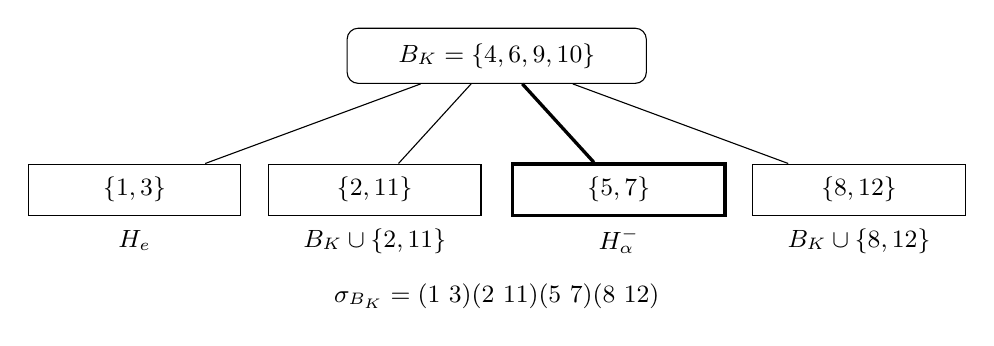
\begin{tikzpicture}[x=1cm,y=1cm, every node/.style={font=\small}]
 \node[draw,rounded corners,minimum width=3.8cm,minimum height=.7cm]
  (b) at (0,0) {$B_K=\{4,6,9,10\}$};
 \node[draw,minimum width=2.7cm,minimum height=.65cm]
  (p1) at (-4.6,-1.7) {$\{1,3\}$};
 \node[draw,minimum width=2.7cm,minimum height=.65cm]
  (p2) at (-1.55,-1.7) {$\{2,11\}$};
 \node[draw,very thick,minimum width=2.7cm,minimum height=.65cm]
  (p3) at (1.55,-1.7) {$\{5,7\}$};
 \node[draw,minimum width=2.7cm,minimum height=.65cm]
  (p4) at (4.6,-1.7) {$\{8,12\}$};
 \draw (b) -- (p1); \draw (b) -- (p2);
 \draw[very thick] (b) -- (p3); \draw (b) -- (p4);
 \node at (-4.6,-2.35) {$H_e$};
 \node at (-1.55,-2.35) {$B_K\cup\{2,11\}$};
 \node at (1.55,-2.35) {$H^-_\alpha$};
 \node at (4.6,-2.35) {$B_K\cup\{8,12\}$};
 \node at (0,-3.05)
  {$\sigma_{B_K}=(1\ 3)(2\ 11)(5\ 7)(8\ 12)$};
\end{tikzpicture}
\caption{La estrella concreta de la bandera dodecafásica. Cada línea
indica la unión de la cuaterna central con el par de su extremo; la
línea gruesa señala la hexada seleccionada también por los signos
anteriores al acarreo de $\alpha$. Los cuatro pares agotan las ocho
posiciones exteriores.}
\label{exc:fig-estrella}
\end{figure}

\begin{proposition}[La familia de estrellas]
\label{exc:m12}
Las $\binom{12}4=495$ permutaciones $\sigma_B$ preservan $\mathcal H$.
El grupo que generan tiene orden $95040$ y es el grupo de Mathieu
$M_{12}$ en su acción sobre el pequeño diseño de Witt.
\end{proposition}

\begin{proof}
La preservación se reduce a la definición~\ref{exc:codigo}. Se recorren las
$3^6$ palabras $c(w)=(w,wA_W)$, se retienen los $132$ soportes de peso seis
y, para cada $B\in\binom{[12]}4$, se forman los cuatro pares
$H\setminus B$ con $B\subset H$. Esos pares particionan
$[12]\setminus B$; la sustitución de cada coordenada por su pareja envía
de nuevo los $132$ soportes sobre sí mismos. Esta verificación finita prueba
\(\{\sigma_B(H):H\in\mathcal H\}=\mathcal H\) para las $495$ cuaternas.

Seis estrellas suficientes para la generación son las siguientes; la
segunda columna exhibe la cuaterna fijada por cada permutación:
\[
\begin{array}{c|c|l}
i&B_i&g_i=\sigma_{B_i}\\ \hline
1&\{1,2,3,4\}&(5\ 12)(6\ 11)(7\ 9)(8\ 10)\\
2&\{1,2,3,5\}&(4\ 12)(6\ 10)(7\ 11)(8\ 9)\\
3&\{1,2,3,6\}&(4\ 11)(5\ 10)(7\ 8)(9\ 12)\\
4&\{1,2,4,5\}&(3\ 12)(6\ 9)(7\ 8)(10\ 11)\\
5&\{1,3,4,5\}&(2\ 12)(6\ 8)(7\ 10)(9\ 11)\\
6&\{2,3,4,5\}&(1\ 12)(6\ 7)(8\ 11)(9\ 10).
\end{array}
\tag{M12.1}
\label{eq:exc-seis-estrellas-m12}
\]
Sea $G_i=\langle g_1,\ldots,g_i\rangle$. Su clausura finita queda
determinada por
\[
 G_i^{(0)}=\{1\},\qquad
 G_i^{(n+1)}=G_i^{(n)}\cup
 \{g_jh:1\leq j\leq i,\ h\in G_i^{(n)}\},\qquad
 G_i=\bigcup_{n\geq0}G_i^{(n)}.
\tag{M12.2}
\label{eq:exc-clausura-finita-m12}
\]
La estabilización de esta recurrencia da
\[
\begin{array}{c|rrrrrr}
i&1&2&3&4&5&6\\ \hline
|G_i|&2&6&18&360&7920&95040.
\end{array}
\tag{M12.3}
\label{eq:exc-ordenes-generadores-m12}
\]
Una segunda comprobación fija sucesivamente los puntos $1,2,3,4,5$. Para
$G=G_6$ se obtiene
\[
\begin{array}{c|rrrrrr}
\text{puntos fijados}&0&1&2&3&4&5\\ \hline
|G_{(1,\ldots,k)}|&95040&7920&720&72&8&1\\
\text{tamaño de la órbita siguiente}&12&11&10&9&8&\text{---}
\end{array}
\tag{M12.4}
\label{eq:exc-cadena-estabilizadores-m12}
\]
Las entradas de \eqref{eq:exc-ordenes-generadores-m12} y
\eqref{eq:exc-cadena-estabilizadores-m12} se obtienen exclusivamente por
composición de las listas de imágenes de
\eqref{eq:exc-seis-estrellas-m12}; por órbita--estabilizador, su producto
es $12\cdot11\cdot10\cdot9\cdot8=95040$.

Como cada $g_i$ preserva $\mathcal H$, se tiene
$G\leq\operatorname{Aut}(\mathcal H)$. La unicidad de la hexada que
contiene una quíntupla y la enumeración incidencial de la
definición~\ref{exc:codigo} hacen trivial el estabilizador puntual de una
quíntupla; por consiguiente,
$|\operatorname{Aut}(\mathcal H)|\leq
12\cdot11\cdot10\cdot9\cdot8$. La igualdad de órdenes prueba
$G=\operatorname{Aut}(\mathcal H)$ y la pertenencia de las $495$ estrellas
a $G$. El grupo de automorfismos del sistema $S(5,6,12)$ así obtenido es,
por definición y reconocimiento de su acción natural, el grupo de Mathieu
$M_{12}$.
\end{proof}

Una estrella individual genera un grupo cíclico de orden dos. No
genera por sí sola $M_{12}$, y menos aún el Monstruo. Tampoco la
existencia de $495$ generadores de un grupo de permutaciones prueba que
cada uno sea el transporte de un lazo específico del TPK. Esa afirmación
requiere el mapa de lazos correspondiente; el resultado aquí establecido
es la acción incidencial finita.

\begin{remark}[La igualdad de trazas no identifica operadores]
Sobre $V_{11}$, una estrella tiene espectro $+1$ con multiplicidad siete
y $-1$ con multiplicidad cuatro. Su traza normalizada es $3/11$.
Un proyector de rango tres en el mismo espacio tiene también traza
normalizada $3/11$, pero espectro $1^3,0^8$. No son conjugados: sus
polinomios mínimos y sus espectros son diferentes. El entrelazador
\eqref{exc:incidencia} transporta operadores definidos; no convierte
esta coincidencia escalar en una equivalencia de operadores.
\end{remark}

\subsection{El residuo binario y las cinco regiones de \texorpdfstring{$\pi$}{pi}}
\label{exc:cinco-regiones}

El siguiente reconocimiento utiliza el código de Golay binario
extendido $G_{24}$, de parámetros $[24,12,8]_2$. Sus pesos son
$0,8,12,16,24$, y los soportes de peso ocho forman el diseño
$S(5,8,24)$. Fijamos una dodecada $D$, soporte de una palabra de peso
doce. Este dato y el isomorfismo de incidencia que se declarará a
continuación pertenecen a la carta de realización; no se usan para
generar ni seleccionar los decimales de $\pi$.

\begin{proposition}[Residuo de una dodecada y elevación de hexadas]
\label{exc:residuo-binario}
El conjunto
\[
 \mathcal H(D)=
 \{O\cap D: O\text{ es una octada},\ |O\cap D|=6\}
\]
es un sistema $S(5,6,12)$ sobre $D$. Cada una de sus hexadas tiene
una única elevación a una octada. Para cualquier cuaterna $B\subset D$,
las cinco octadas que la contienen se distribuyen en cuatro elevaciones
residuales y una única octada $O_B^\perp$ con $O_B^\perp\cap D=B$.
\end{proposition}

\begin{proof}
Una quintupla $A\subset D$ pertenece a una única octada $O$. Si
$j=|O\cap D|$, la palabra binaria suma de $O$ y $D$ tiene peso
$20-2j$. Entre los pesos permitidos, y con $0\leq j\leq8$, sólo
son posibles $j=2,4,6$. Como $A\subset O\cap D$, se tiene $j\geq5$
y por tanto $j=6$. Esto da existencia y unicidad de la hexada
residual, así como unicidad de su elevación al escoger cinco de sus
puntos. Por otra parte,
\[
 \lambda_4(S(5,8,24))=\frac{\binom{20}1}{\binom41}=5,
 \qquad
 \lambda_4(S(5,6,12))=4.
\]
Las cuatro hexadas residuales sobre $B$ dan cuatro octadas distintas.
La quinta no puede cortar $D$ en seis puntos, pues sería otra hexada
residual; como contiene $B$, su intersección tiene tamaño cuatro y
coincide con $B$.
\end{proof}

Una carta $\ell:[12]\to D$ que preserve las hexadas identifica
$\mathcal H$ con $\mathcal H(D)$. Su existencia es el reconocimiento
del diseño ya construido como el pequeño diseño de Witt; una elección
concreta de $\ell$ fija el relabelado. La elevación
\[
 \iota_D:\mathcal H\longrightarrow
       \{\text{octadas de }G_{24}\},
 \qquad H\longmapsto O\text{ tal que }O\cap D=\ell(H),
\]
es inyectiva porque la intersección con $D$ recupera $\ell(H)$.
Esta inyectividad tiene por dominio las hexadas, no el registro $K$.

La relación con las cinco regiones de $\pi$ conserva datos más ricos
que el número cinco. Las emisiones y sus firmas son:
\begin{center}
\small
\begin{tabular}{@{}crll@{}}
\toprule
Región & Multiplicidad & Emisión $U_6$ & Firma \\
\midrule
$\perp$ & $432$ & $(501,614,498,169,272,272)$ & $555555$ \\
$++_1$ & $144$ & $(810,923,870,169,272,272)$ & $339555$ \\
$++_2$ & $144$ & $(810,983,810,169,272,272)$ & $393555$ \\
$++_3$ & $144$ & $(870,923,810,169,272,272)$ & $933555$ \\
$--$ & $144$ & $(870,923,810,418,674,521)$ & $933717$ \\
\bottomrule
\end{tabular}
\end{center}
En cada bloque decimal de tres cifras, la firma usa la diferencia
modular de las dos primeras cifras. Las cinco emisiones tienen la
misma palabra trítica visible $w_\pi=010211$, pero no la misma
genealogía regional. Las tres regiones positivas conservan la cola
$169|272|272$; la región negativa la cambia por $418|674|521$;
la región transversal tiene firma constante y multiplicidad mayor.

La extensión marcada de la carta regional envía la región transversal
a $O_{\ell(B_K)}^\perp$, la negativa a $\iota_D(H^-_\alpha)$ y las
tres positivas a las otras tres elevaciones de la estrella. Así se
realiza la partición $4+1$ de las cinco octadas sobre $\ell(B_K)$.
La correspondencia individual entre los tres nombres positivos y
los tres pétalos restantes exige un orden de carta; no la determina
la incidencia sin ese dato. Por ello la afirmación precisa es una
correspondencia de regiones marcada, compatible con sus roles y con
la bandera, no una biyección canónica deducida del cardinal cinco.

La identidad $432+4\cdot144=1008$ conserva las multiplicidades
regionales. También $1008=36\cdot28$ y una octada tiene
$\binom82=28$ parejas. Estas igualdades son controles aritméticos de
catálogo, no sustitutos del mapa $\iota_D$ ni de la carta regional.

\subsection{Del código ternario al retículo de Niemeier}
\label{exc:niemeier}

El paso a dimensión veinticuatro no necesita recorrer primero el
código binario. Se realiza directamente desde $C_W$ por pegado de
discriminantes. Así quedan distinguidas dos prolongaciones compatibles:
una conserva el residuo $W_{12}\subset W_{24}$; la otra construye el
retículo sobre el que se realizará el álgebra de operadores de vértice.

Sea $A_2=\mathbb Z a_1\oplus\mathbb Z a_2$ con matriz de Gram
\[
 \begin{pmatrix}2&-1\\-1&2\end{pmatrix},
 \qquad \rho=a_1+a_2,\qquad \rho^2=2.
\]
Representamos las tres clases de $A_2^*/A_2$ mediante
\[
 \varpi_0=0,\qquad
 \varpi_1=\frac{2a_1+a_2}{3},\qquad
 \varpi_2=\frac{a_1+2a_2}{3}.
\]
La aplicación $j\mapsto\varpi_j+A_2$ identifica aditivamente
$\mathbb F_3$ con ese discriminante. Para $c\in C_W$, escribimos
$\phi(c)=(\varpi_{c_1},\ldots,\varpi_{c_{12}})$ y definimos
\begin{equation}
 N(C_W)=\bigcup_{c\in C_W}\bigl(A_2^{12}+\phi(c)\bigr).
 \label{exc:niemeier-def}
\end{equation}

\begin{theorem}[Pegado ternario]
\label{exc:niemeier-teorema}
El objeto \eqref{exc:niemeier-def} es un retículo positivo, par y
unimodular de rango $24$. Su sistema de raíces es exactamente
$A_2^{12}$; por tanto, se reconoce como el retículo de Niemeier con
ese sistema de raíces.
\end{theorem}

\begin{proof}
La linealidad del código hace que la unión de clases sea estable por
suma. La autoortogonalidad anula el emparejamiento discriminante:
éste es un múltiplo de $c\cdot d/3$ módulo $\mathbb Z$. Así, el
retículo es integral. La norma de una clase de pegado es
$2\operatorname{wt}(c)/3$ módulo $2\mathbb Z$. Los pesos de
\eqref{exc:enumerador} son múltiplos de tres, de modo que es par.

El índice de $A_2^{12}$ en $N(C_W)$ es $|C_W|=3^6$. En consecuencia,
\[
 \det N(C_W)=\frac{3^{12}}{(3^6)^2}=1.
\]
La positividad procede de la suma ortogonal de las doce métricas $A_2$.
En una clase no nula de $A_2^*/A_2$ la norma mínima es $2/3$;
toda palabra no nula tiene al menos seis posiciones no nulas.
Por tanto, un vector de una clase de pegado no trivial tiene norma
al menos $6\cdot2/3=4$. No aparecen raíces de norma dos fuera de
$A_2^{12}$. Dentro de éste, las raíces son precisamente las de sus
doce componentes.
\end{proof}

\subsection{Selección incidencial del vecino unimodular sin raíces}
\label{exc:leech}

La etiqueta $o_*=1$ de la bandera se realiza ahora como una de las
doce componentes $A_2$. Esta operación declara la métrica anterior y
la cámara radial positiva
\[
 v(a)=\sum_{i=1}^{12}a_i\rho_i,
 \qquad a_i=1+3b_i,\quad b_i\in\mathbb Z_{\geq0}.
\]
El requisito de paridad del vecino de índice tres es
$v(a)^2\equiv0\pmod{18}$. Puesto que
\[
 v(a)^2=2\sum_i(1+3b_i)^2,
\]
esa congruencia equivale a $\sum_i b_i\equiv1\pmod3$. El menor
valor de la norma en la cámara se obtiene con un único $b_i=1$ y
todos los demás nulos; es $54$. El origen marcado selecciona
\begin{equation}
 v_\alpha=4\rho_1+\rho_2+\cdots+\rho_{12},
 \qquad v_\alpha^2=54.
 \label{exc:vector}
\end{equation}
La palabra ``menor'' se refiere a esta cámara positiva. No afirma
minimalidad en toda la clase residual: el vector
$(a_1-2a_2,\rho,\ldots,\rho)$ representa la misma clase módulo tres
y tiene norma $14+11\cdot2=36$. La restricción de cámara es parte
de los datos de la construcción, no una conclusión omitible.

Sea $N=N(C_W)$. Definimos
\begin{equation}
 N_{\alpha,0}=\{x\in N:\langle x,v_\alpha\rangle\equiv0\pmod3\},
 \qquad
 N_\alpha=N_{\alpha,0}+\mathbb Z\frac{v_\alpha}{3}.
 \label{exc:vecino}
\end{equation}

\begin{theorem}[Vecino de Leech determinado por la bandera marcada]
\label{exc:teorema-leech}
Con la métrica y la cámara declaradas, $N_\alpha$ es un retículo
positivo, par y unimodular de rango $24$, sin vectores de norma dos.
Por el teorema de clasificación correspondiente, es isométrico al
retículo de Leech $\Lambda_{24}$.
\end{theorem}

\begin{proof}
El carácter $x\mapsto\langle x,v_\alpha\rangle\bmod3$ no es nulo:
una raíz simple de una componente se empareja con $a_i\rho_i$ en
$a_i\equiv1\pmod3$. Por ello $[N:N_{\alpha,0}]=3$ y
$\det N_{\alpha,0}=9$. Además,
$v_\alpha/3\in N_{\alpha,0}^*$ y $v_\alpha\in N_{\alpha,0}$.
Si $v_\alpha/3$ perteneciera a $N$, la integridad de $N$ haría que
todos los emparejamientos con $v_\alpha$ fueran divisibles por tres,
contradiciendo el carácter no nulo. La clase de $v_\alpha/3$ tiene
por tanto orden tres. Se deduce
\[
 [N_\alpha:N_{\alpha,0}]=3,
 \qquad \det N_\alpha=9/3^2=1.
\]
La extensión es integral, y para $x\in N_{\alpha,0}$,
\[
 \left(x+m\frac{v_\alpha}{3}\right)^2
   =x^2+2m\frac{\langle x,v_\alpha\rangle}{3}+6m^2
   \in2\mathbb Z.
\]
Luego es par.

Queda excluir las raíces, que es el paso decisivo. Las raíces de $N$
pertenecen a $A_2^{12}$. Sus emparejamientos con $v_\alpha$ son
congruentes con $\pm1$ o $\pm2$ módulo tres; ninguna pertenece a
$N_{\alpha,0}$. Para las otras dos clases del vecino, cada componente
pertenece a alguna de las clases locales
\[
 A_2+\varpi_j\pm\rho/3,\qquad j=0,1,2.
\]
Como $4\rho/3\equiv\rho/3\pmod{A_2}$, esta descripción vale
también en la componente distinguida. Escribiendo un vector local
como $(u a_1+v a_2)/3$, su norma es
$2(u^2-uv+v^2)/9$. Las seis clases anteriores tienen residuos no
nulos y mínimo $2/9$: los representantes de mínima forma cuadrática
son $(\pm1,0),(0,\pm1),(1,1),(-1,-1)$ en los residuos apropiados.
Un vector de una clase nueva tiene, por tanto, norma al menos
$12\cdot2/9=8/3>2$. No hay raíces en ninguna de las tres clases.
La clasificación de los retículos pares unimodulares positivos de
rango veinticuatro identifica el único caso sin raíces con
$\Lambda_{24}$.
\end{proof}

El argumento no reconoce Leech por una coincidencia de dimensión.
Construye el pegado, prueba integridad, paridad y determinante, y
elimina las raíces mediante una cota local. Sólo entonces aplica el
teorema de clasificación. La dependencia de $\alpha$ se conserva en
la bandera que selecciona $o_*$ y en el vector \eqref{exc:vector};
no se convierte el valor escalar de la constante en una longitud del
retículo.

\subsection{El álgebra de operadores de vértice y el Monstruo}
\label{exc:voa}

Sea $\Lambda=N_\alpha$, ya reconocido como Leech. El paso siguiente
utiliza su retículo integral, no una expansión decimal. La construcción
de álgebra de operadores de vértice de retículo se escribe
\[
 V_\Lambda=M(1)\otimes\mathbb C_\varepsilon[\Lambda].
\]
Aquí $M(1)$ es el espacio de osciladores de Heisenberg en rango
veinticuatro; $\mathbb C_\varepsilon[\Lambda]$ es el álgebra de grupo
torcida por el cociclo de la extensión central del retículo. El
cociclo y el levantamiento de las isometrías forman parte de la
construcción: una suma vectorial desnuda no determina los productos
de vértice.

La negación $\lambda\mapsto-\lambda$ admite el levantamiento estándar
$\theta$. Con su módulo torcido y la elección de paridad compatible,
la construcción de Frenkel--Lepowsky--Meurman produce
\begin{equation}
 V^\natural_{\rm HMT}
   =V_\Lambda^+\oplus(V_\Lambda^T)^+.
 \label{exc:flm}
\end{equation}
El signo $+$ denota la parte par de la acción levantada. La expresión
incluye el producto de vértice del orbifold; no se limita a una suma
de espacios graduados.

\begin{theorem}[Prolongación hasta el módulo Moonshine]
\label{exc:moonshine}
El álgebra \eqref{exc:flm}, construida sobre el vecino
\eqref{exc:vecino}, es una realización del álgebra Moonshine
$V^\natural$. Tiene carga central $24$, componente de peso uno nula
y grupo de automorfismos isomorfo al Monstruo $\mathbb M$. Su carácter
graduado es
\begin{equation}
 \operatorname{Tr}_{V^\natural_{\rm HMT}}q^{L_0-1}
   =J(\tau)=j(\tau)-744
   =q^{-1}+196884q+21493760q^2+\cdots,
 \qquad q=e^{2\pi i\tau}.
 \label{exc:j}
\end{equation}
\end{theorem}

\begin{proof}
El teorema \ref{exc:teorema-leech} verifica las hipótesis reticulares:
positividad, paridad, unimodularidad, rango veinticuatro y ausencia de
raíces. Se aplica entonces la construcción y el teorema de
Frenkel--Lepowsky--Meurman para el retículo de Leech. Éstos identifican
el orbifold con $V^\natural$, establecen su carácter y su grupo de
automorfismos. La composición de la bandera, el vecino y el functor
de construcción de VOA da la realización aquí indicada. No se deduce
el grupo a partir del coeficiente $196884$.
\end{proof}

El teorema utilizado es un reconocimiento clásico posterior con
hipótesis verificadas, no una nueva demostración en este artículo de
la construcción FLM \cite{flm}.
Además, la notación $q=e^{2\pi i\tau}$ es la variable convencional
de Fourier empleada para reconocer el carácter. No introduce $\pi$
ni $e$ como entradas del generador coinductivo que ya los ha determinado.

Puede verse una parte del mecanismo de traza antes del orbifold.
Sólo el vector reticular cero queda fijo por la negación; cada
oscilador contribuye con signo alterno. De ahí
\[
 \operatorname{Tr}_{V_\Lambda}\theta q^{L_0-1}
   =t_2(\tau)
   :=q^{-1}\prod_{n\geq1}(1+q^n)^{-24}.
\]
Esta traza en el álgebra de retículo no debe confundirse con el
carácter sin inserción de $V^\natural$. Tampoco identifica por sí
sola una clase de conjugación del Monstruo: el espacio, la inserción
y el levantamiento deben especificarse antes de comparar funciones.

\subsection{Trazas graduadas de Moonshine y representación del Monstruo}
\label{exc:alcance}

Para $g\in\operatorname{Aut}(V^\natural_{\rm HMT})$, la traza
con inserción es
\[
 T_g(\tau)=
 \operatorname{Tr}_{V^\natural_{\rm HMT}}gq^{L_0-1}.
\]
El teorema de Moonshine monstruoso identifica estas series como
Hauptmoduln de los grupos de género cero correspondientes
\cite[teorema~1.1]{borcherds}.
El carácter $J$, el grupo $\mathbb M$ y la familia $g\mapsto T_g$
son realizaciones del álgebra ya construida. No forman una sucesión
causal en la que primero se adivina $J$ y después se deduce el Monstruo.

La unidad tiene aquí una localización algebraica precisa. El subespacio
de peso cero es la línea del vacío, \(V^\natural_0=\CC\mathbf1\), y
el coeficiente de \(q^{-1}\) de \(J\) es por ello \(1\). En peso uno
la dimensión es cero, de donde procede la ausencia del término constante
en \(J=j-744\). Un morfismo de álgebras de vértices conserva el vector
vacío. Esta propiedad proporciona el sentido técnico de conservación
de la unidad en este nivel; la unidad de los observables cilíndricos
se conserva por la precomposición demostrada anteriormente. La relación
entre ambos niveles debe seguir los mapas de construcción con sus unidades.

En peso dos aparece la igualdad
\[
 196884=1+196883=196560+324=54(5\cdot729+1).
\]
La primera separación corresponde a la línea conforme trivial y al
componente irreducible de dimensión $196883$ de la representación
del Monstruo. Las otras expresiones tienen lecturas reticulares o
aritméticas. Su igualdad no identifica automáticamente sus sumandos
con regiones, palabras o rutas del TPK. Para hacerlo habría que
presentar los mapas entre esos espacios y probar que respetan las
acciones relevantes.

\newpage
En particular, una isometría $N_\alpha\simeq\Lambda_{24}$ induce
una realización de \eqref{exc:flm}, y una elección de isomorfismo
con $V^\natural$ transporta su grupo de automorfismos. No se ha
construido con ello una acción del Monstruo sobre los dígitos de
$\pi$, sobre los bloques de $K$ o sobre todas las historias TPK.
Tal afirmación adicional requeriría una representación
$\rho_{\rm TPK}$ y un mapa $F$ con un cuadrado explícito
\[
 F\rho_{\rm TPK}(g)=\rho_{V^\natural}(g)F,
\]
incluyendo dominio, codominio e información conservada. La ausencia
de ese paso en la afirmación presente no retira el entrelazador
incidencial $U_W$, la bandera ni el vecino ya construidos; sólo
delimita una promoción distinta, de acción sobre el estado fuente.

La cadena establecida en esta sección puede resumirse, manteniendo
visibles sus datos de transporte, como
\begin{align*}
 &\text{APP--TRIT--TPK y estado aritmético con memoria de trayectoria}
   \longrightarrow (w_j,f_j;K,s_0)\\
 &\longrightarrow (C_W,\mathcal H;B_K\subset H^-_\alpha,
                   P_\pi,H_e,H_\varphi,H_{\rm APP})\\
 &\longrightarrow \bigl(N(C_W),o_*,\text{métrica y cámara}\bigr)
   \longrightarrow N_\alpha
   \longrightarrow V^\natural_{\rm HMT}.
\end{align*}
En el nivel de incidencia, las estrellas generan $M_{12}$ y la
carta residual realiza la estructura regional $4+1$ en $W_{24}$.
En el nivel reticular y de VOA, la construcción da Leech y el módulo
Moonshine. Son prolongaciones de una misma fuente marcada, con
objetos y mapas diferentes. La continuidad causal no obliga a
identificar sus codominios ni a borrar las elecciones explícitas
de marco, cámara y levantamiento.

El resultado de la sección es una derivación reunida: las pruebas finitas,
incidenciales, reticulares y vertex-operatoriales realizan el tránsito desde
la incidencia dodecafásica hasta las hipótesis de los teoremas de
reconocimiento. En los dominios y con las elecciones de carta declarados,
la cadena construye el diseño de Witt, genera su grupo de Mathieu, selecciona
el vecino de Leech y prolonga la estructura hasta el módulo Moonshine; cada
etapa conserva el objeto, la operación y la información transportada que
hacen aplicable el reconocimiento posterior.

\clearpage
\input{sections/v_accion_estructural.tex}
\clearpage
\section{Coordenadas angulares y observables del borde}
\input{sections/v_coordenadas_angulares.tex}
\clearpage
\input{sections/v_funcional_barbero.tex}
\clearpage
\input{sections/gravedad_rigidez_20260926.tex}
\clearpage
\input{sections/v_unidad_areal.tex}
\input{sections/evaluacion_gravitatoria_20260926.tex}
\clearpage
\input{sections/v_area_informacion.tex}
\clearpage
\input{sections/v_transduccion_termica.tex}
\clearpage
\input{28_portador_tensorial.tex}
\clearpage
\input{29_retorno_y_memoria_traslacional.tex}
\clearpage
\input{30_pantalla_y_respuesta.tex}
\clearpage
\input{30d_realizacion_geometrica.tex}
\clearpage
\part*{II. Amplitud, evolución y persistencia}
\addcontentsline{toc}{part}{II. Amplitud, evolución y persistencia}
\input{30b_variacion_energia_memoria.tex}
\clearpage
\input{30c_composicion_corriente_conexion.tex}
\clearpage
\input{30e_corriente_extension_minima.tex}
\clearpage
\input{31_corriente_y_respuesta_cartan.tex}
\clearpage
\input{32_eliminacion_torsional_no_lineal.tex}
\clearpage
\input{33_corriente_espinorial_y_densidad.tex}
\clearpage
\input{50_dilucion_y_rebote.tex}
\clearpage
\input{51_solucion_homogenea.tex}
\clearpage
\input{60_tensor_residual_y_balance.tex}
\clearpage
\part*{III. Horizontes y respuesta relacional}
\addcontentsline{toc}{part}{III. Horizontes y respuesta relacional}
\input{70_horizontes_e_informacion.tex}
\clearpage
\input{80_observador_y_respuesta_relacional.tex}
\clearpage
\input{81_propagacion_bidireccional.tex}
\clearpage
\input{90_conclusiones.tex}
